
\documentclass[11pt]{article}
\usepackage{makecell}
\usepackage[a4paper]{geometry}
\geometry{left=2.0cm,right=2.0cm,top=2.5cm,bottom=2.5cm}

\usepackage{ctex}
\usepackage{amsmath,amsfonts,graphicx,subfigure,amssymb,bm,amsthm}
\usepackage{algorithm,algorithmicx}
\usepackage{subfigure} 
\usepackage[noend]{algpseudocode}
\usepackage{fancyhdr}
\usepackage{mathrsfs}
\usepackage{mathtools}
\usepackage[framemethod=TikZ]{mdframed}
\usepackage{fontspec}
\usepackage{adjustbox}
\usepackage{breqn}
\usepackage{fontsize}
\usepackage{tikz,xcolor}
\usepackage{geometry}
\usepackage{setspace}
\usepackage{xeCJK}
\usepackage{ulem}
\usepackage{pstricks}
\usepackage{pstricks-add}
\usepackage{breqn}
\usepackage{esint}
\usepackage{textcomp}
\usepackage{upgreek}
\usepackage{pifont}
\usepackage{circuitikz}
\usepackage{caption}
\usepackage{multirow}
\usepackage{diagbox}
\usepackage{hyperref}
\usepackage{cite}
\usepackage{authblk}
\usepackage{listings}
\usepackage{xcolor}
\usepackage{pythonhighlight}
\setmainfont{Palatino Linotype}


\title{基于人像分割的实时虚拟背景替换系统}  

\renewcommand*{\Authsep}{,}
\renewcommand*{\Authand}{,}
\renewcommand*{\Authands}{,}


\author{马俊程}
\author{魏昕原}
\author{屈泽凯}
\author{郦运琛}
\affil{{\small2021K8009929021},{\small2021K8009915002},{\small2021K8009916005},{\small2021K8009929028}}


\begin{document}
\date{}
	\maketitle
\section{问题分析}

由于我们组对语义分割领域较感兴趣,在本次大作业自主选题,选择“虚拟背景”作为题目,希望训练出一个轻量级高精度的人像分割模型,实现实时虚拟背景替换。

虚拟背景广泛应用于视频会议、在线教育等场景中,可以消除背景噪声、保护隐私或者提升视频质量,从而来增强用户体验。虚拟背景的一种实现方案为,通过将人像与背景分割开,然后将人像放置在虚拟背景中,这本质上是一个语义分割任务。但因虚拟背景的应用场景多为移动设备,对实时性和轻量化的要求较高,高精度语义分割模型无法胜任,需要轻量化的实时语义分割模型。同时,由于虚拟背景只需要将人与背景分割开,具有自己的先验特征,出现了一些针对人像分割的模型。
	\begin{figure}[!h]
  \centering
  \subfigure[]{
  \begin{minipage}[t]{0.2\linewidth}
  \centering
  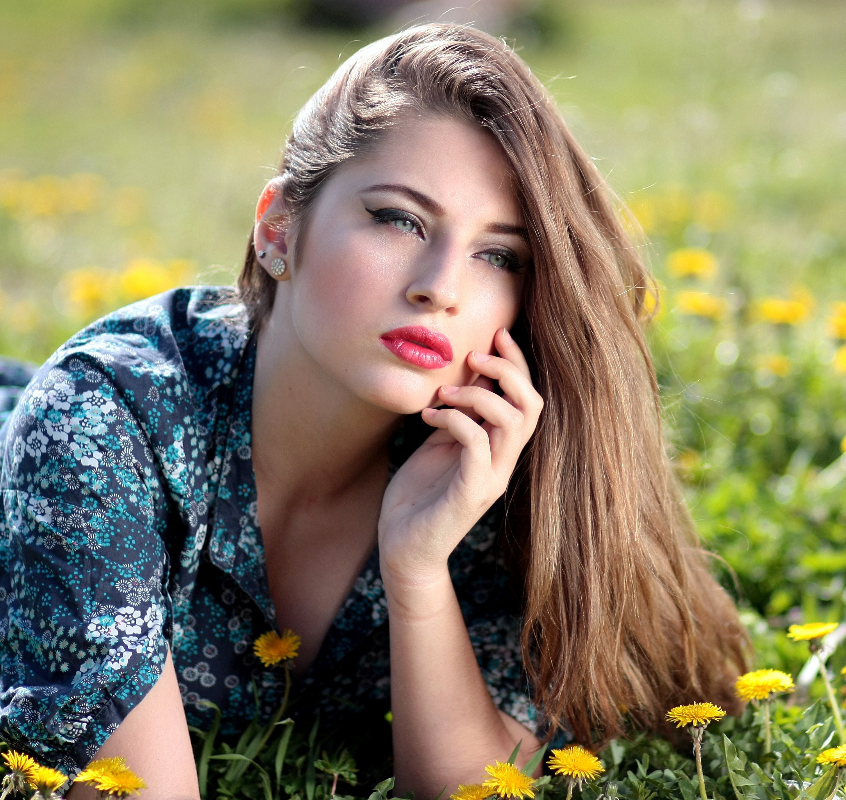
\includegraphics[width=1\linewidth]{a1.jpg}
  %\caption{fig1}
  \end{minipage}%
  }%
  \subfigure[]{
  \begin{minipage}[t]{0.2\linewidth}
  \centering
  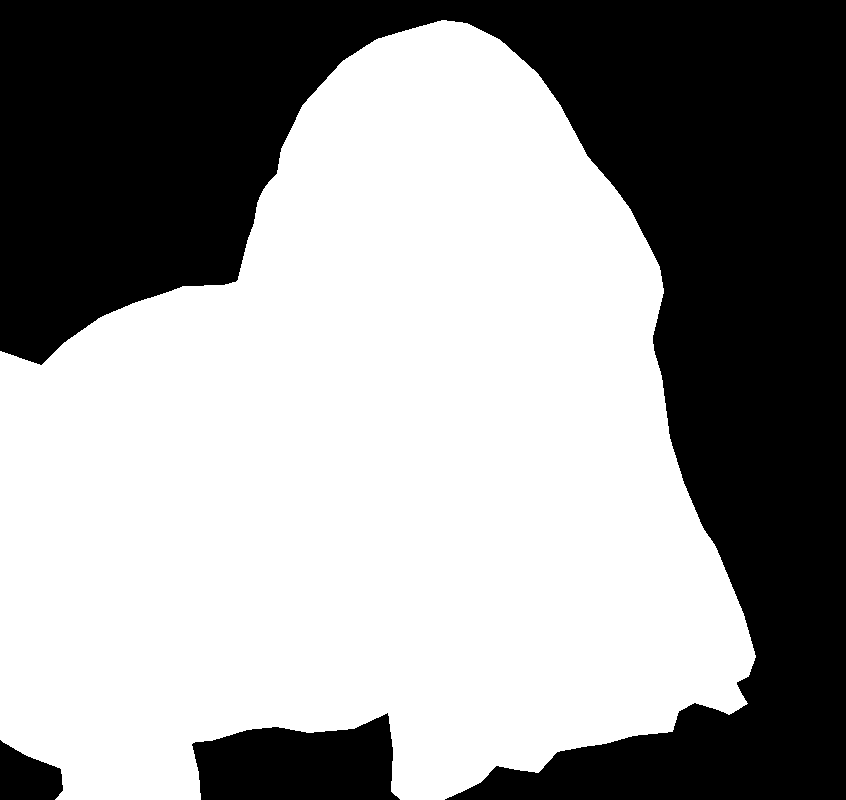
\includegraphics[width=1\linewidth]{a2.png}
  %\caption{fig2}
  \end{minipage}%
  }%
  \subfigure[]{
  \begin{minipage}[t]{0.2\linewidth}
  \centering
  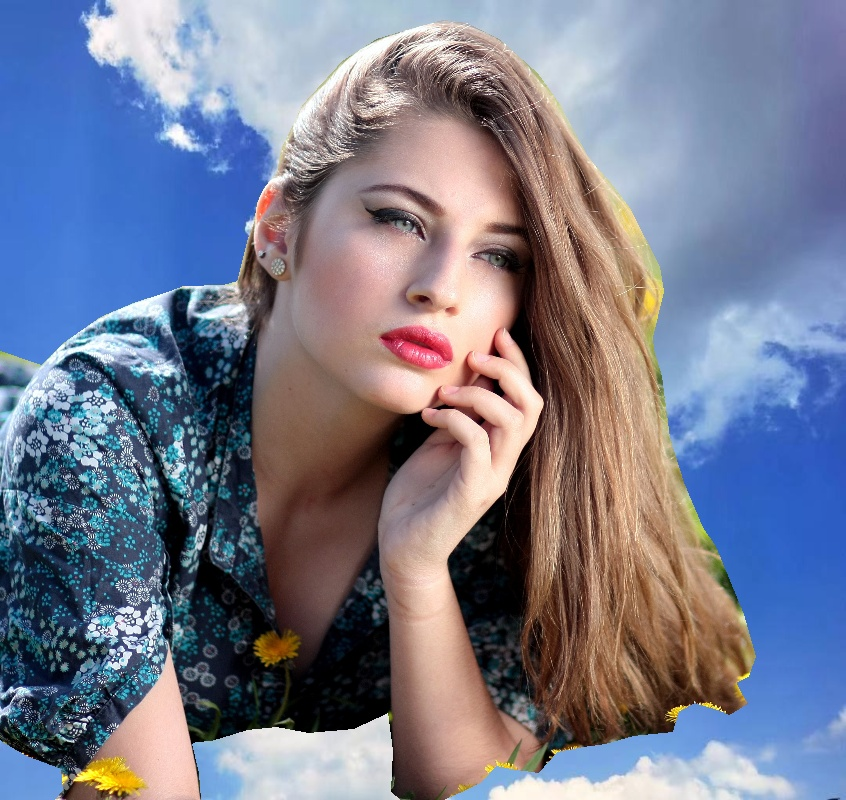
\includegraphics[width=1\linewidth]{a3.jpg}
  %\caption{fig2}
  \end{minipage}%
  }%
  \subfigure[]{
  \begin{minipage}[t]{0.2\linewidth}
  \centering
  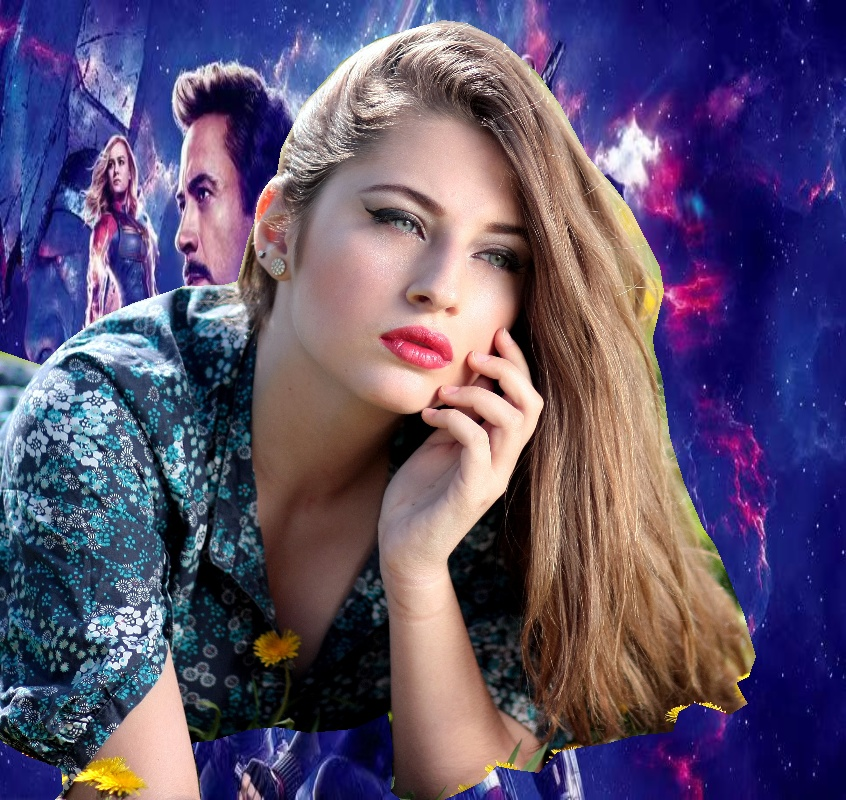
\includegraphics[width=1\linewidth]{a4.jpg}
  %\caption{fig2}
  \end{minipage}%
  }%

  \subfigure[]{
  \begin{minipage}[t]{0.2\linewidth}
  \centering
  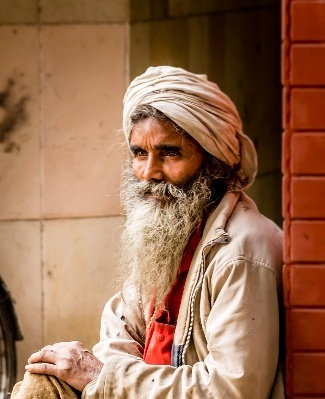
\includegraphics[width=1\linewidth]{b1.jpg}
  %\caption{fig2}
  \end{minipage}%
  }%
  \subfigure[]{
  \begin{minipage}[t]{0.2\linewidth}
  \centering
  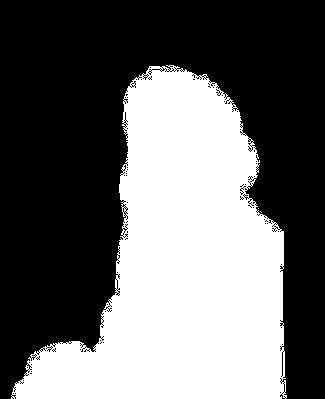
\includegraphics[width=1\linewidth]{b2.png}
  %\caption{fig2}
  \end{minipage}%
  }%
  \subfigure[]{
  \begin{minipage}[t]{0.2\linewidth}
  \centering
  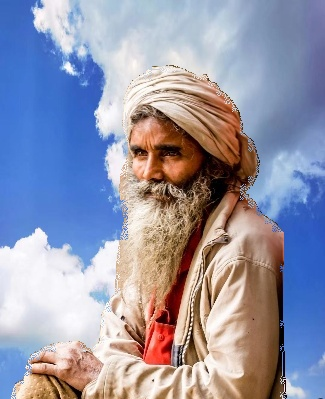
\includegraphics[width=1\linewidth]{b3.jpg}
  %\caption{fig2}
  \end{minipage}%
  }%
  \subfigure[]{
  \begin{minipage}[t]{0.2\linewidth}
  \centering
  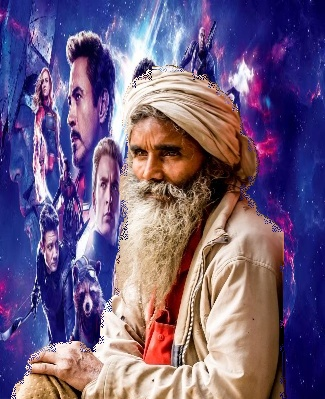
\includegraphics[width=1\linewidth]{b4.jpg}
  %\caption{fig2}
  \end{minipage}%
  }%
  \centering
  \caption{虚拟背景替换。(a)(e)为原图;(b)(f)为人像分割的掩码图;(c)(g)和(d)(h)为背景替换后的图片}
\end{figure}

	语义分割是计算机视觉领域的一项基本任务,旨在将图像中的每个像素都分配给特定的语义类别,例如人、车、路、树等等。随着深度学习技术的发展,特别是卷积神经网络(CNN)的出现,语义分割技术得到了快速发展。早期语义分割模型大多是基于全卷积网络的编码器解码器结构,例如FCN\cite{ref1}、SegNet\cite{ref2}、UNet\cite{ref3}等。后来,出现了应用空洞卷积的DeepLab系列模型\cite{ref4},利用了空洞卷积的特点,能够在保证分辨率的同时扩大感受野。近两年,涌现出一批应用了transformer的高精度语义分割模型,如SETR\cite{ser},Segmenter\cite{segm}等。
	
	随着移动设备需求的增大,许多工作开始针对实时语义分割设计轻量级模型。相比于高精度语义分割方法,实时语义分割需要满足更高的速度和实时性要求,并且在尽可能少的时间内完成分割任务,追求最高的精度-效率平衡。这一领域有两种主流方法,基于编码器-解码器结构的ENet\cite{ref7}、SFNet\cite{ref34}等,和基于双多分支结构的BiSeNet\cite{ref6}、Pidnet\cite{ref41}等。
	
	人像分割是语义分割的一个子问题,目标类别只有作为前景的人和背景两种。和通用语义分割相比,人像分割具有额外的挑战,如实时性,重视边界的分割精度等。人像分割的发展历程也与深度学习技术的进步密切相关。最早的人像分割方法主要基于传统算法,如基于边缘检测和区域生长的方法。然而,这些方法的准确度和鲁棒性受到限制,尤其是在复杂场景中。近年来,许多基于深度学习的人像分割算法被提出,如PortraitNet\cite{porn},SiNet\cite{ref43}等。
	
	我们搜索了人像分割领域公开的数据集并对其进行整理,得到下表。结合数据集的大小和复杂程度,我们选择在Supervise-Portrait数据集上进行实验,最终在Supervise-Portrait、EG1800和PP-HumanSeg14K数据集上训练。
	\begin{center}
		\begin{tabular}{p{1.5cm}p{7cm}p{4cm}}
			\hline
			数据集名称&网络链接&数据集简介 \\ \hline
			Maadaa&\makecell{https://maadaa.ai/dataset/\\live-streamer-portrait-segmentation/}&照片张数:15.6K张;分辨率:$540\times960 \sim 720\times1280$,为人体和背景的分割。\\ \hline
			AISeg&\makecell{$https://github.com/aisegmentcn/$\\$matting\_human\_datasets$}&包含34427张图像和对应的matting结果图,经过人脸检测和区域裁剪后生成了600*800的半身人像。\\ \hline
			EG1800&\makecell{https://aistudio.baidu.com/aistudio/\\datasetdetail/155370}&包含了1736张图片和对应的label,分辨率:$512\times512 \sim 512\times1024$ \\ \hline
			PP-HumanSeg14K&\makecell{https://github.com/PaddlePaddle/\\PaddleSeg}&包含来自291个会议场景的23个视频,帧为14K,分辨率:$1280\times720$包含各种电话会议场景、参与者动作、照明变化。\\ \hline
			Supervise-Portrait&https://github.com/dong-x16/PortraitNet&PortraitNet作者从集Supervisory.ly精心挑选的人像分割数据集,具有比EG1800更复杂的背景。\\\hline
		\end{tabular}
	\end{center}

	我们将在报告中给出完整的虚拟背景替换方案,先通过人像分割模型给出人像的掩码,再使用后处理模块实现背景替换,整体流程如图\ref{fig:net}所示。我们主要做出了以下贡献

\textit{i)针对人像分割任务,我们设计了基于非对称编码器-解码器的模型,在Supervise-Portrait数据集上实现了最佳的精度-效率平衡,凭借0.248M参数达到95.95\% mIoU,以最高的精度和最低的参数量超过其他实时分割模型。并且,我们的模型具有良好的泛化能力,将最终模型直接在EG1800数据集上训练,便得到95.74\% mIoU,与其他人像分割模型相比,实现了最佳精度-效率平衡。将baseline直接在PP-HumanSeg14K上训练,不改变任何结构和超参数,即可在验证集上达到94.59\% mIoU,超过百度PP-Humanseg论文中的94.2\%。}

\textit{ii)我们设计了多尺度上下文模块SAPPM,具有强大的提取和聚合全局信息的能力,超过其他高效上下文模块。我们提出了流对齐-注意力融合模块,可以对齐不同分辨率特征图的语义信息,实现高效的特征融合。}

\textit{iii)我们完成了完整的背景替换系统,设计了后处理模块,利用膨胀、腐蚀、光流等图像处理方法,使替换背景后的图像更加自然。并且,我们利用PyQt5实现了实时演示系统。}

\begin{figure}[H]
  \centering
  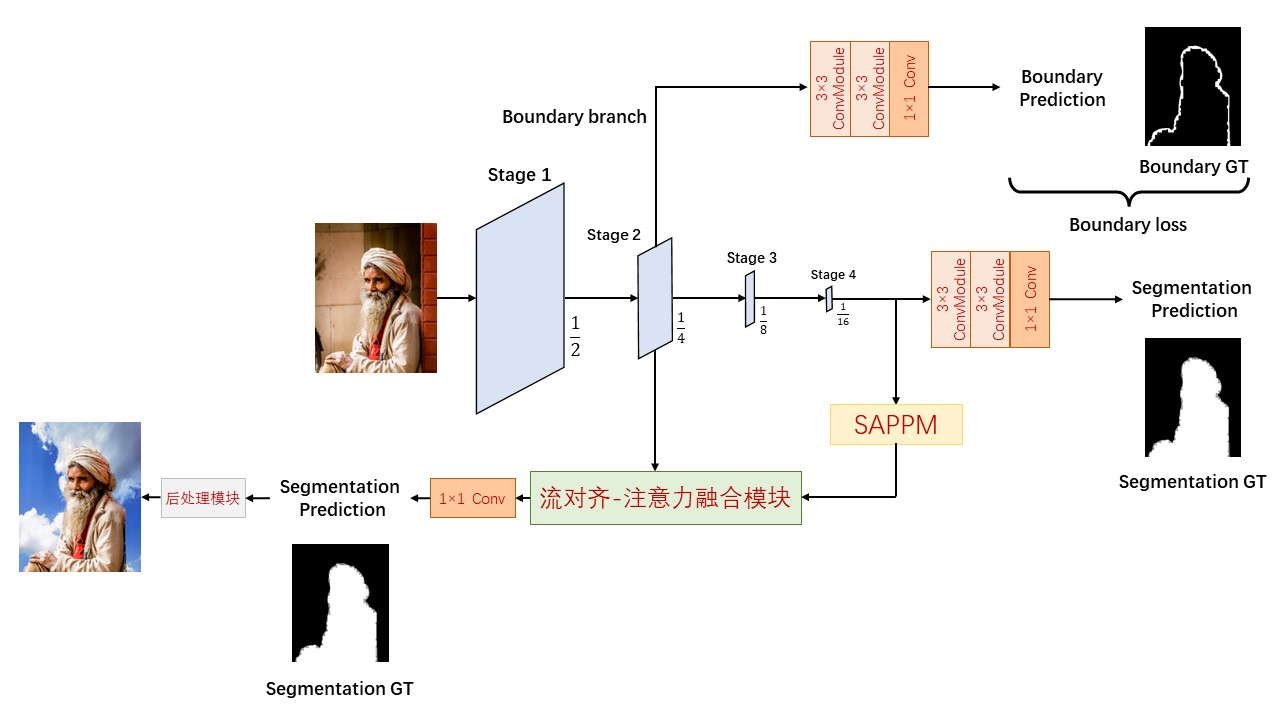
\includegraphics[width=15cm]{net.jpg}
  \caption{整体结构}
  \label{fig:net}
\end{figure}

\section{相关工作调研}
我们组将使用人像分割的方法实现虚拟背景任务,而人像分割作为语义分割的一个子领域,在实际应用时对实时性有较高的要求。因此,我们在这一部分将分别讨论基于监督学习的语义分割、实时语义分割和人像分割三个方面的相关工作。


\subsection{语义分割}
语义分割作为计算机视觉领域的基础任务之一,具有长久的发展历史。在深度学习方法流行之前,基于传统机器学习分类器的语义分割方法使用较多。但传统方法需要手工设计特征,无法使用一些深层和隐藏的特征,这导致图像特征的使用受到限制,在深度学习流行起来后很快被超过。
我们在这一部分将简要介绍基于深度学习的语义分割方法,并分为基于CNN和基于Transformer两部分分别讨论。
\subsubsection{基于CNN的语义分割}
由于深度学习的快速发展,一系列深度神经网络取得了巨大的成就,特别是卷积神经网络,如 VGG \cite{VGG}、GoogLeNet\cite{goo}、ResNet\cite{res}等。这些网络的出现为语义分割带来了新的解决方案。基于卷积神经网络的方法具有天然的优势,它可以自动提取语义特征,而不是原来方法中有偏差的人工特征提取。并且是端到端的处理结构,预测图可以直接在输出层得到。 

和分类任务不同,语义分割作为一种密集预测任务需要对每个像素进行预测,因此,高层次的语义信息和低层次的细粒度信息对精度都有重要影响。语义信息为预测提供上下文特征,可以考虑全局对象的长距依赖,提供非局部的视角。它一般通过CNN下采样(跨步卷积,池化等)提取,在这个过程中特征图的分辨率不断降低,感受野不断增大,高层次的语义信息被编码到特征中。
但只有语义信息无法给出精确的分割结果,因为每个像素点的局部特征在下采样的过程中逐渐丢失,无法给出精细的预测。包含空间结构信息的细粒度特征对分割边界的精度很重要,较浅卷积层的高分辨率特征图往往被认为含丰富的细粒度特征。
由于分割任务的特殊性,感受野与分辨率、语义特征与细粒度特征之间往往存在矛盾,语义分割工作大多围绕细粒度特征和上下文特征的提取和融合展开。本部分将按照提出的方法,对相关工作分类进行介绍。


\paragraph{编码器-解码器结构}
\textbf{FCN}\cite{ref1} 是第一个将CNN用于语义分割的工作,仅包含卷积层,使其能够接受任意大小的图像并生成相同大小的分割图。通过使用跳跃连接,其中来自模型最后一层的特征图被上采样并与较早阶段的特征图融合,从而结合了语义信息和细粒度信息,得到了不错的精度,被视为语义分割的一个里程碑。
\begin{figure}[H]
    \centering
    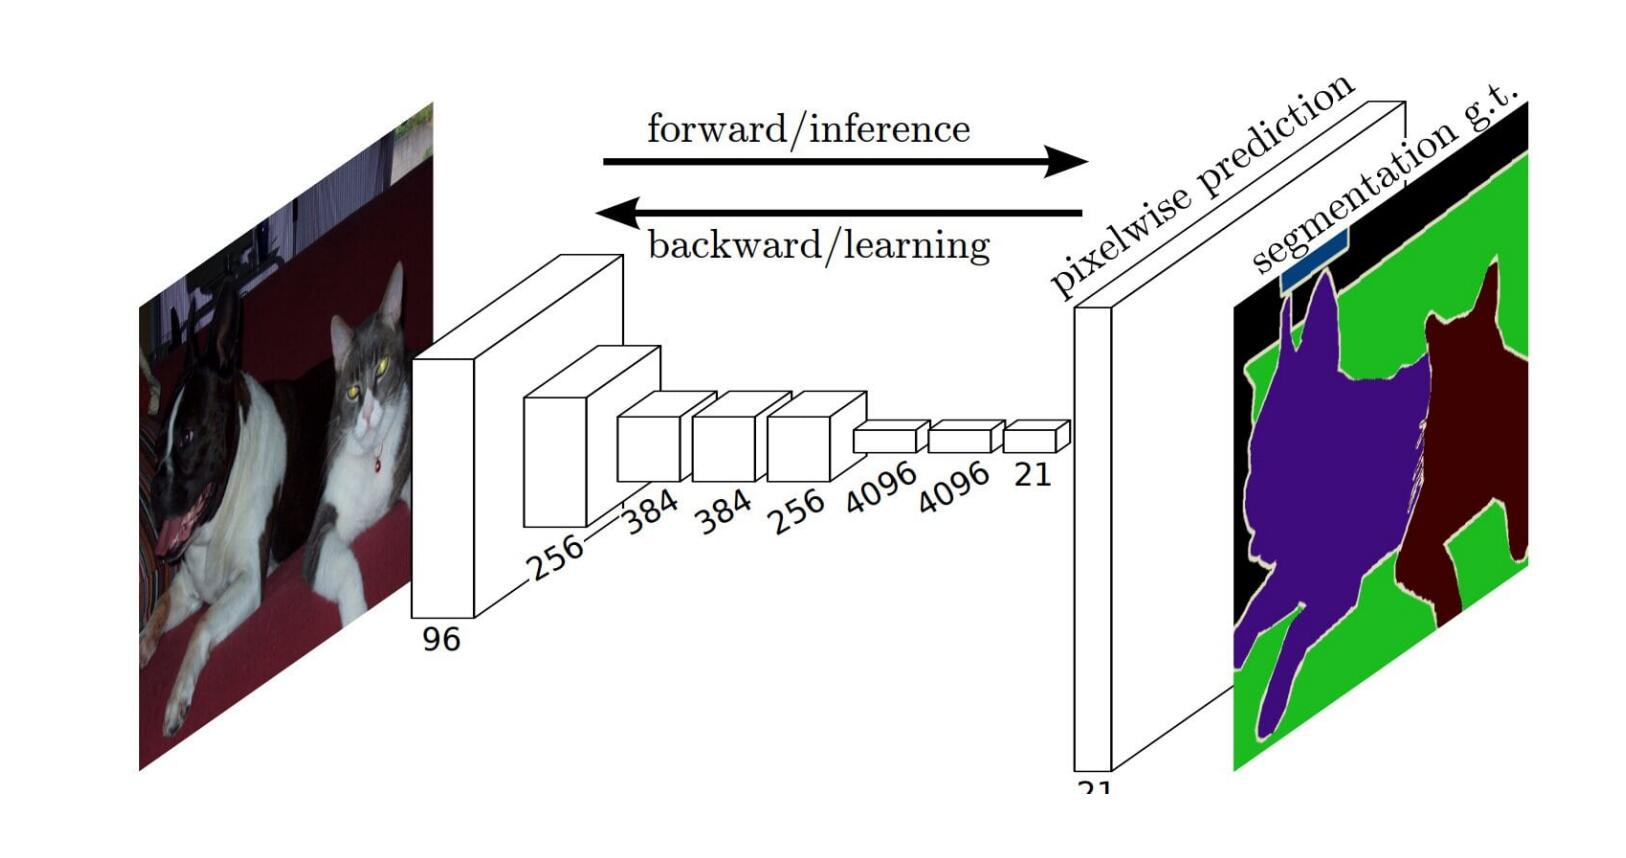
\includegraphics[width=9cm]{fig1.jpg}
    \caption{FCN\cite{ref1}}
\end{figure}

\textbf{U-Net}\cite{ref3} 最初为用于医学图像的分割模型,但后来广泛取得优秀结果,是经典的编码器-解码器结构。它由两部分组成,编码器部分采用了全卷积网络,通过下采样获得一系列特征图,将得到的低分辨率但富含语义信息的特征图输入解码器进行上采样,每次上采样都会将结果与下采样过程中对应的特征
图裁剪后拼在一起,从而在这个过程中多次聚合语义特征和细粒度特征,实现很好的效果。由于上采样和下采样过程比较对称,形成一个U型结构,故起名为U-Net。

\begin{figure}[H]
    \centering
    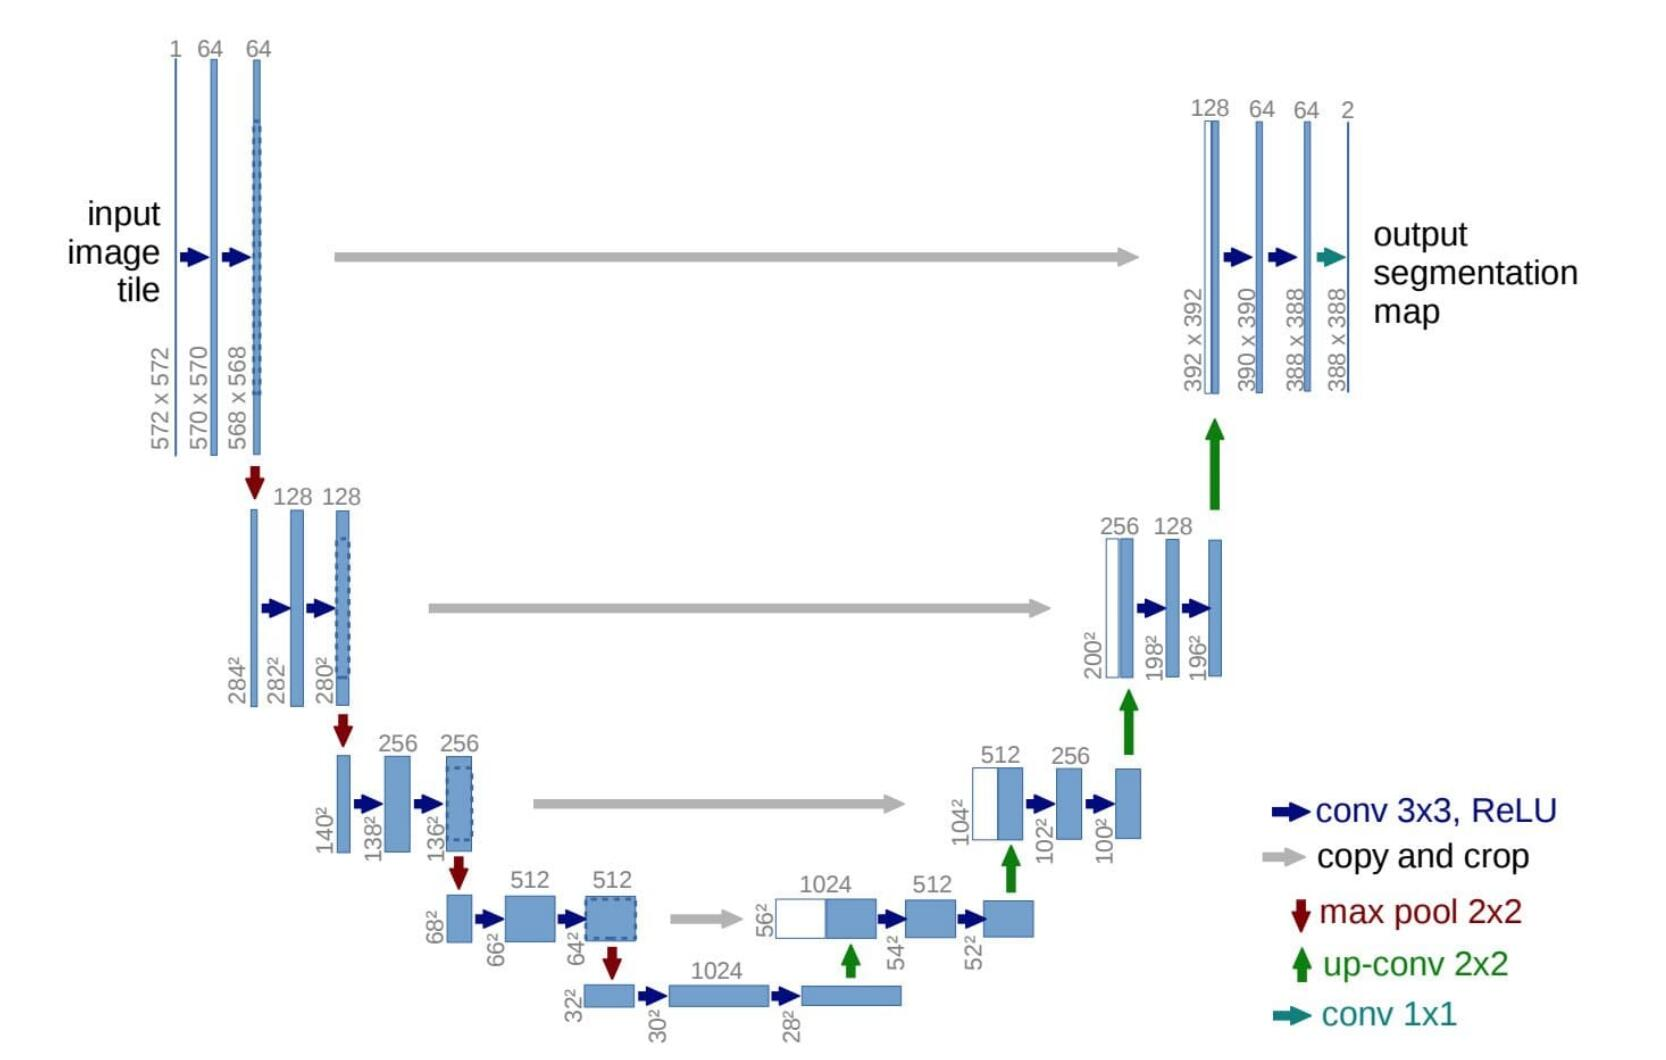
\includegraphics[width=10cm]{fig2.jpg}
    \caption{U-net\cite{2021INet}}
\end{figure}

\textbf{Segnet}\cite{ref2}提出最大反池化,创新了上采样的方式,即解码器使用相应编码器中最大池化时计算的池化索引来进行上采样,上采样后的图经过卷积层可产生密集的特征图。与反卷积相比,这种方式不需要学习,大大减小了计算量,并且只需要储存下采样时的最大池化索引而非特征图,节省了内存。

\paragraph{空洞卷积}
扩张卷积(Dilated convolution,又称空洞卷积,atrous convolution)在卷积层中引入了另一个参数,即扩张率。例如,一个3×3的核,如果扩张率为2,那么它将具有与5×5的核相同的感受野大小,但只使用了9个参数,从而在不增加计算成本的情况下扩大了感受野。
\begin{figure}[H]
    \centering
    \subfigure[]{
    \begin{minipage}[t]{0.5\linewidth}
    \centering
    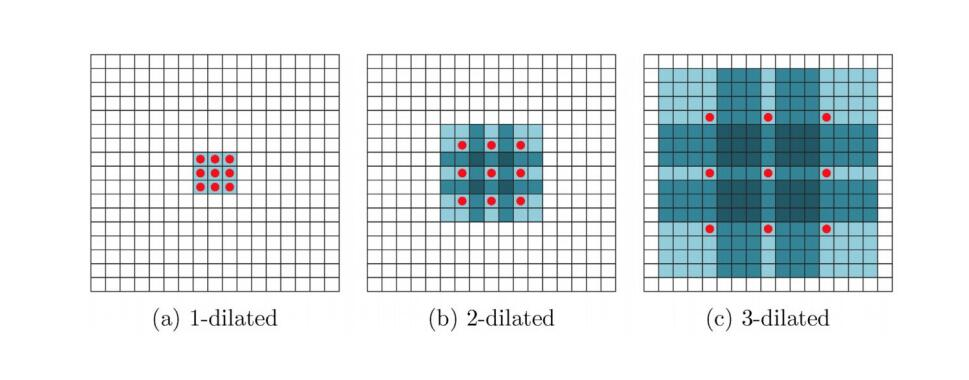
\includegraphics[width=6cm]{fig7.jpg}
    %\caption{fig1}
    \end{minipage}%
    }%
    \subfigure[]{
    \begin{minipage}[t]{0.5\linewidth}
    \centering
    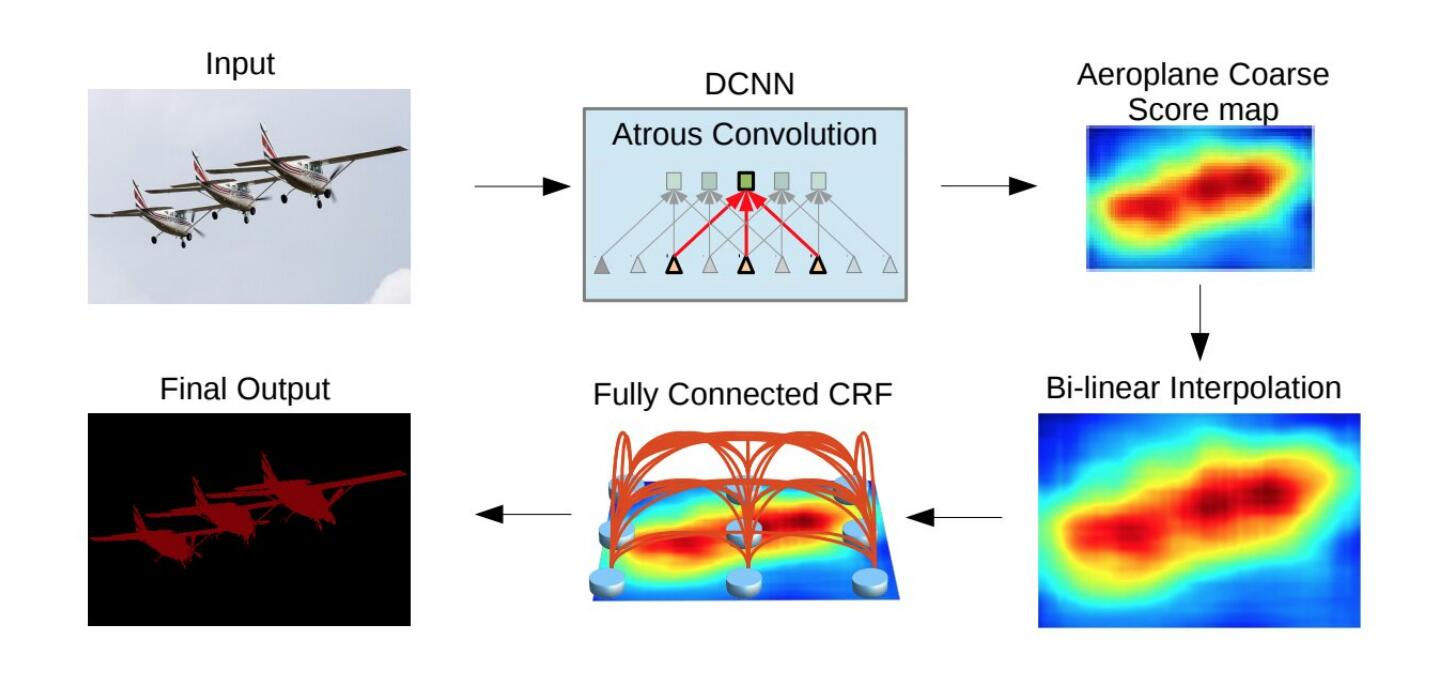
\includegraphics[width=6cm]{fig6.jpg}
    %\caption{fig2}
    \end{minipage}%
    }%
    \centering
    \caption{(a)空洞卷积原理;(b)Deeplab\cite{ref4}}
\end{figure}


扩张卷积可以在保持分辨率的同时增大感受野,在语义分割中应用广泛。\textbf{DeepLab}\cite{de1,ref4,de3,de3+}系列网络用空洞卷积改造主干网络,使下采样后的特征图保持一个较高的分辨率,并提出一个提取多尺度上下文特征的ASPP模块,得到了很好的精度。



\paragraph{上下文模块}
由于分割的目标有不同的尺寸,许多工作设计了提出多尺度上下文的模块。
\textbf{PSPNet} \cite{2016Pyramid}提出金字塔池化模块,能更好地学习场景的全局上下文表示。这个网络使用残差网络(ResNet)作为特征提取器,其中应用了空洞卷积,从输入图像中提取不同模式的特征。这些特征图被送入金字塔池化模块,它们在四个不同的尺度上进行池化,获得不同尺度的上下文特征。

\begin{figure}[H]
    \centering
    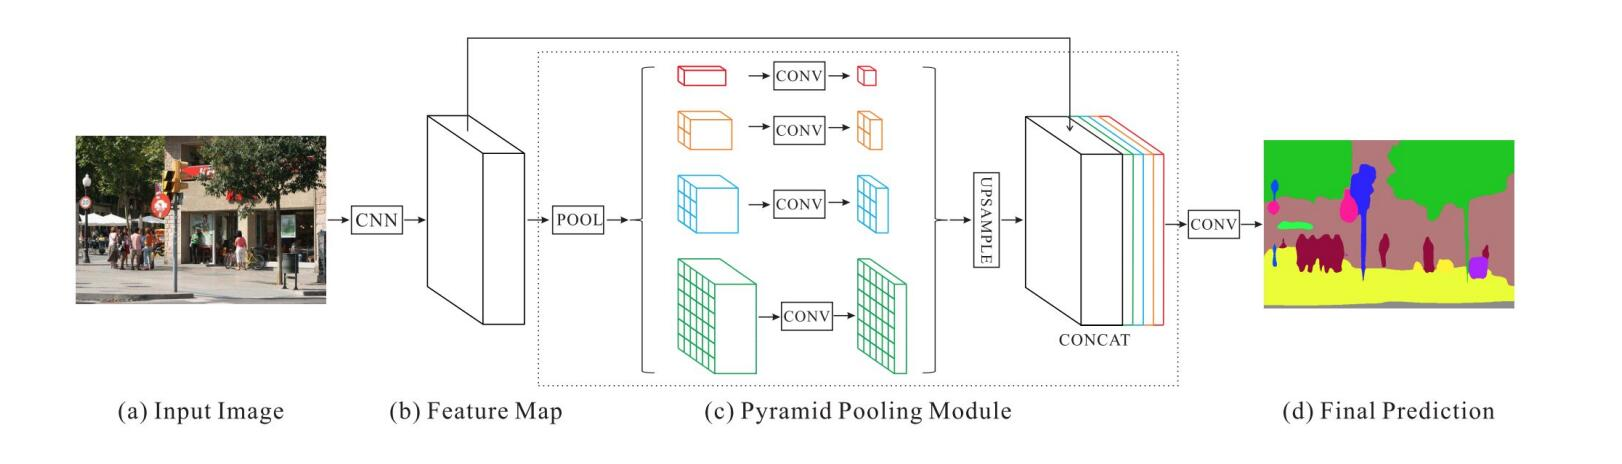
\includegraphics[width=10cm]{fig5.jpg}
    \caption{PSPNet\cite{2016Pyramid}}
\end{figure}

注意力机制在捕获长程依赖性,提取全局特征上具有强大的优势,并且自注意力具有全局感受野,许多工作将注意力模块加入语义分割模型,获得了不错的效果。

\textbf{EncNet}\cite{enc}提出了一个CEM(Context Encoding Module)模块,编码上下文信息,再对特征图的每个通道加权。\textbf{PSANet}\cite{psa}引入逐点注意力,考虑全局相关性,每个点都自适应的通过一个可学习的注意力映射与其他所有点连接起来。\textbf{Non-local}\cite{non}将非局部的方法归纳成一个范式,并提出简化的自注意力操作。
\textbf{DANet}\cite{dan}为了更好的捕捉上下文信息(全局信息)和通道间的联系,提出了一种双注意力网络,分别提取空间注意力和通道注意力得到更好的特征表示。

\begin{figure}[H]
    \centering
    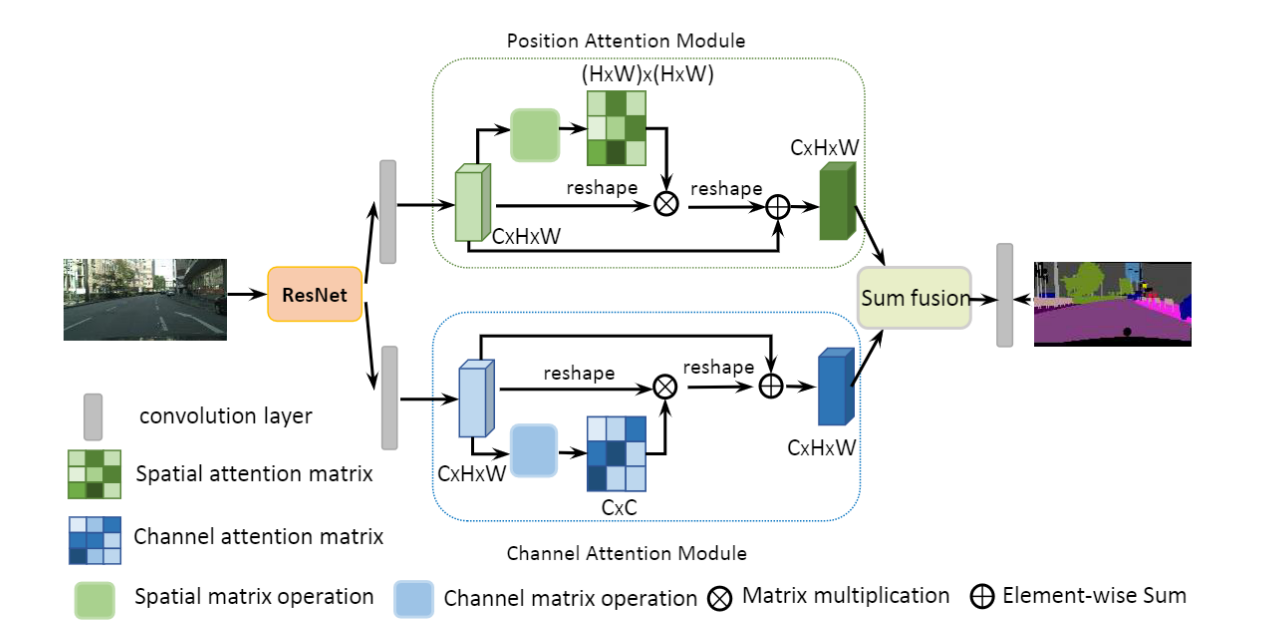
\includegraphics[width=10cm]{dan.png}
    \caption{DANet\cite{dan}}
\end{figure}

由于自注意力的平方复杂度,出现了一系列简化计算的工作,例如\textbf{CCNet}\cite{ccn}仅在当前行和列计算注意力,\textbf{ANN}\cite{ann}先对对K和V进行降维再计算注意力,\textbf{GCNet}\cite{gcn}使用共享注意力图。

\subsubsection{基于Transformer的语义分割}
Transformer首先在自然语言处理领域取得巨大成功\cite{trans},ViT\cite{vit} 遵循 NLP 中的 Transformer 设计第一个Vision Transformer ,可以在图像分类中实现sota,之后又涌现了许多基于 Vision Transformer的主干网络,如Swin Transformer\cite{swi},BEiT\cite{bei},MAE\cite{mae}等,证明了Transformer结构在视觉任务上的优势。
因此,出现了一系列基于Vision Transformer的语义分割工作,取得了强大的效果。

\textbf{SERT}\cite{ser}将ViT应用到语义分割领域,第一个证明了Transformer在此领域的优越性。\textbf{DPT}\cite{dpt}加入了更多卷积特性,对不同Transformer块的输出组装成不同分辨率的类似于图像的形式,
其中较浅层的Transformer块会被组装成更大分辨率的表示,因为其中包含更多细粒度特征,最终融合得到多尺度的特征图。
\textbf{Segmenter}\cite{segm}提出一种新的解码器,学习了多个类嵌入,得到了不错的效果。
\textbf{Segformer}\cite{segf}提出了一种简单高效的基于transformer的语义分割模型,编码时通过合并补丁来获得不同分辨率的特征图,
并使用了一个由全连接层组成的轻量解码器。

\begin{figure}[H]
    \centering
    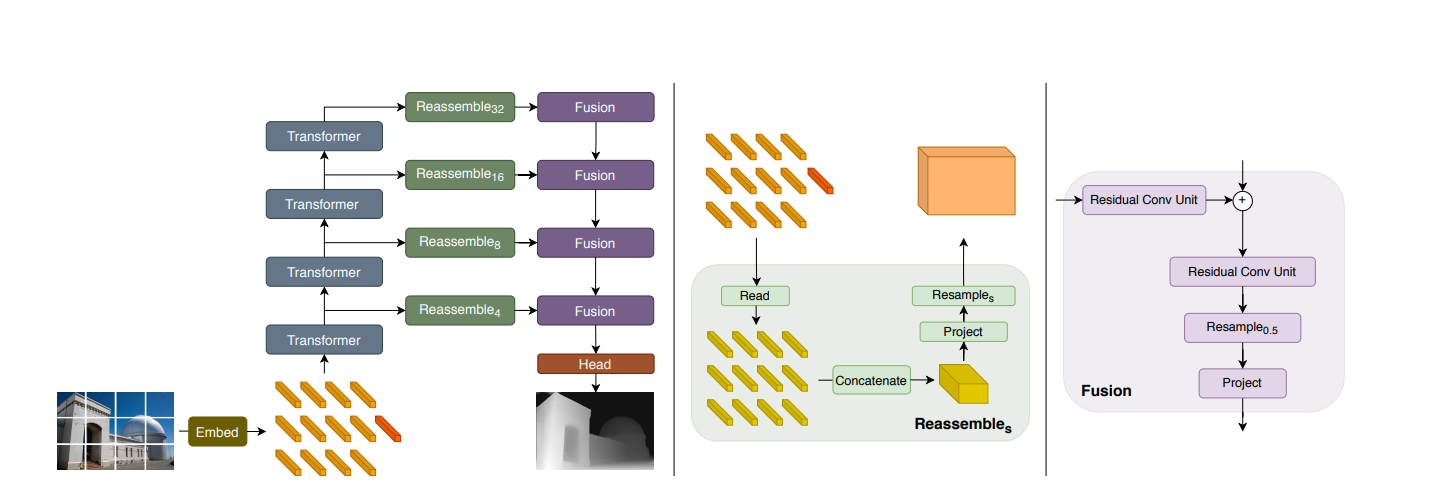
\includegraphics[width=10cm]{dpt.png}
    \caption{DPT\cite{dpt}}
\end{figure}
\subsection{实时语义分割}
在上一部分中提到的语义分割方法使预测的准确度不断提升,但在准确性之外,计算复杂度也是一个重要的考虑因素.现实世界的任务通常旨在在目标平台(硬件)和应用场景(如自动驾驶需要低延迟)给定的有限计算预算下获得最佳精度。
作为机器人和自动驾驶汽车等复杂任务的重要一环,语义分割在许多实际情景中的应用要求它们在内存和计算能力有限的硬件上以非常低的延迟运行,
这激发了一系列针对轻量级架构设计和更好的速度-准确性权衡的工作。

我们将在这一部分沿\textit{i)高效编码器-解码器结构;ii)多分支结构}两个主流方向介绍实时语义分割的相关工作。
\subsubsection{高效编码器-解码器结构}
正如在上一部分中提到的,语义信息和细粒度特征对语义分割任务的精度都十分关键,而编码器-解码器结构是结合这两种特征的一种主要方法。编码器通常为一个特征提取网络,经过多次下采样,特征图的大小逐渐减小,感受野不断扩大,语义特征不断增加。解码器将富含语义信息的特征图经过多次上采样恢复分辨率,并在这个过程中通过横向连接融合细粒度特征,丰富细节信息。
许多实时语义分割工作继续使用了编码器-解码器结构,在保证精度的同时,提出各种方法减小网络的计算量和参数量,使模型轻量化。
\paragraph{高效的主干网络}

许多语义分割模型会选择优秀的主干网络作为编码器,这些主干网络往往针对分类任务设计,并经过了预训练,被认为具有较强的特征提取能力。其中,有一些为移动和资源受限环境设计的轻量级主干,显著减少了所需的操作和内存数量,同时保持较高的准确性。它们的组成模块和高效卷积的方法在实时语义分割任务中广为使用。

\textbf{Mobilenet}\cite{mo1,ref11,ref12}系列网络将深度可分离卷积应用到CNN中,把标准卷积分解为逐深度卷积和逐点卷积。\textbf{Mobilenet V1}\cite{mo1}用深度可分离卷积改进VGG,参数量大大减小的同时,精度仅降低了1\%;\textbf{Mobilenet V2}\cite{ref11}改进了残差块,结合对兴趣流形的分析提出Inverted Residual Block,提高了性能;\textbf{Mobilenet V3}\cite{ref12}利用NAS搜索最优架构,结合其他一些方法(如SE模块)进一步提高了性能。
\textbf{shufflenet}\cite{ref10}使用分组卷积减小1*1卷积层的计算量,并通过通道混合实现组间特征交流;\textbf{shufflenet V2}\cite{ref13}取消了V1的分组卷积,使用通道的分割和混合提高效率。
\textbf{GhostNet}\cite{ref14}减少特征图的固有维数,并通过线性变换生成更多的特征图,在保持相似识别性能的同时降低通用卷积层的计算成本。

\paragraph{设计高效卷积块}

和分类任务相比,语义分割任务作为密集预测任务,还需要多尺度的上下文信息和高分辨率的细节信息。而主干网络通常是为分类任务设计的,其中的卷积块无法完全适应分割任务。因此,许多实时语义分割工作设计了新的轻量化模块,具有更强的提取多尺度特征和细粒度特征的能力。

早期的一些工作利用高效卷积设计新模块,显著降低计算量。\textbf{E-Net}\cite{ref7}是最早地针对实时语义分割的工作之一,它由一个(相对)大编码器和非常简单的解码器组成。整个网络由bottleneck残差块的几种变体构建而成,应用了深度可分离卷积和非对称卷积,上采样时应用了Segnet中的最大反池化方法,实现了一个非常紧凑和快速的架构,可以部署在嵌入式设备上。
\textbf{ErfNet}\cite{ref15}利用不对称卷积改进了基础残差块,相比E-Net提高了精度。\textbf{LEDNet}\cite{ref16}提出SS-nbt块(如图所示),将输入的通道分割后,分别进行非对称卷积和非对称扩张卷积,将结果连接后经残差连接和通道混合得到输出。整体是一个非对称的编码器-解码器结构,在解码器使用特征金字塔,不断细化输出的语义特征。
\begin{figure}[htbp]
    \centering
    \subfigure[]{
    \begin{minipage}[t]{0.20\linewidth}
    \centering
    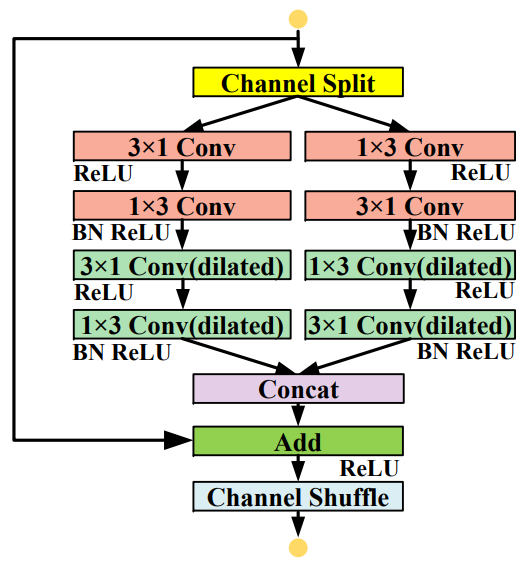
\includegraphics[width=3cm]{led.png}
    %\caption{fig1}
    \end{minipage}%
    }%
    \subfigure[]{
    \begin{minipage}[t]{0.3\linewidth}
    \centering
    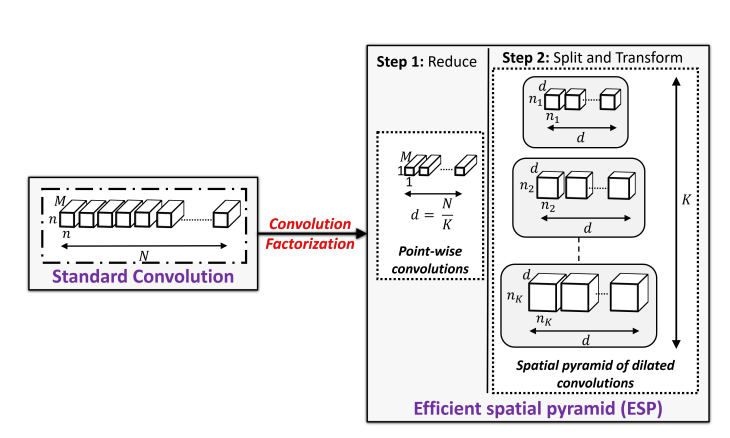
\includegraphics[width=5cm]{esp.png}
    %\caption{fig2}
    \end{minipage}%
    }%
    \subfigure[]{
    \begin{minipage}[t]{0.5\linewidth}
    \centering
    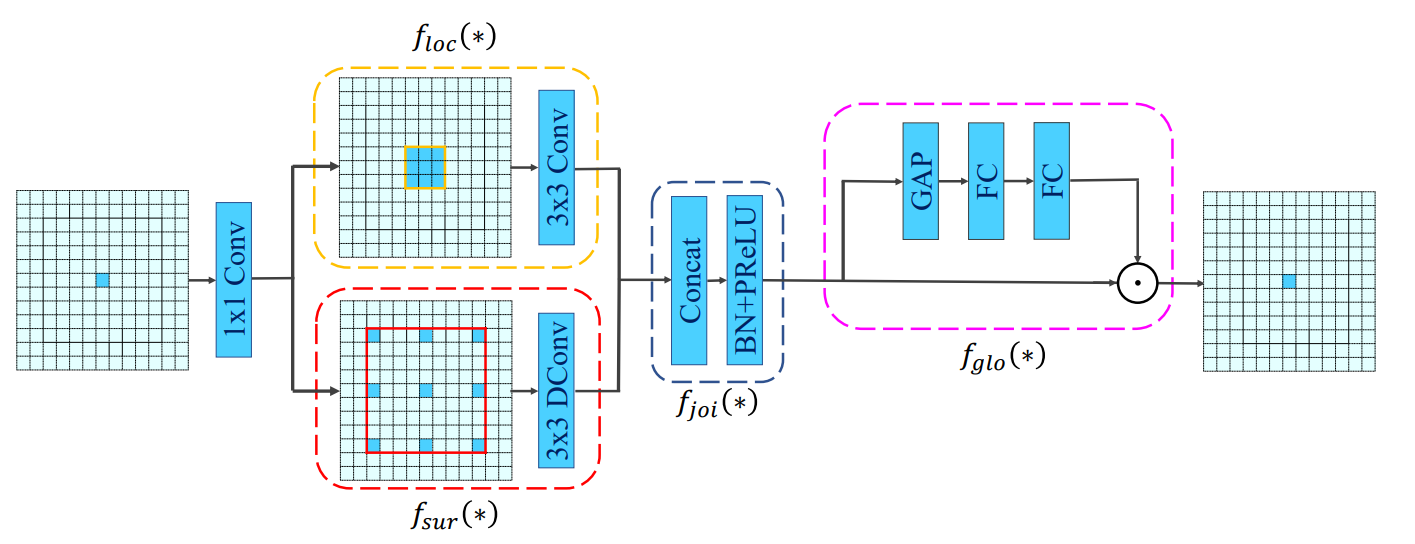
\includegraphics[width=7cm]{cg.png}
    %\caption{fig2}
    \end{minipage}
    }%
    \centering
    \caption{(a)LEDNet\cite{ref16}提出的SS-nbt块;(b)ESPNet\cite{ref17}提出的ESP模块;(c)CGNet\cite{ref19}中提出的CG块}
\end{figure}

许多工作设计了提取上下文信息的高效模块。\textbf{ESPNet}\cite{ref17}提出的高效空间金字塔模块(如图所示),将标准卷积分解,使用1×1卷积降低输入维度,然后使用不同扩张率的并行卷积来增加感受野,提取到多感受野的特征。为了避免由不同的扩张率引起的网格伪影,输出被分层求和,结果被连接起来,最后通过残差连接添加到输入中。\textbf{Espnet V2}\cite{ref18} 在原ESP模块的基础上,使用分组卷积计算1*1卷积,并将空洞卷积改为深度可分离的,大大减小了计算量。
\textbf{CGNet}\cite{ref19}认为在特征提取时需要有上下文信息的指导,设计了CG块(如图所示),以其为主干设计了CGNet,可以在每个阶段融合局部、上下文和全局特征。
\textbf{MSFNet}\cite{ref20}针对高分辨率输入,设计了SAP模块,通过多尺度池化在每个感受野级别都有很好的空间信息恢复,并且将不同感受野层次相同分辨率的特征融合起来,在几乎不增加计算成本的情况下大大提高了性能,并且使用了针对边界的辅助任务,增强模型对边界的敏感度\textbf{RegSeg}\cite{ref21}提出的D块使用通道分割、分组卷积、空洞卷积等方法,还加入了SE模块,融合全局信息。
\textbf{DWRSeg}\cite{ref22}认为选择合适的感受野大小对提取特征的效率很重要,在浅层需要较小的感受野来捕捉局部特征,而高层需要更大的感受野捕捉语义特征,针对感受野设计了DWR块和SIR块。

一些工作改进了融合不同层次特征的方法。\textbf{SF-net}\cite{ref34}认为不同层次提取的特征在语义水平上存在差距,可能导致信息的无效传播。受视频中的“光流”启发,引入了语义流的概念,并提出了一种新颖的基于流的对齐模块(FAM)来学习相邻级别特征图之间的语义流场,用流场修正采样的标准网格,更有效地将高级语义特征融合到高分辨率特征。
\textbf{SFNet-lite}\cite{ref35}在SF-net的基础上,把主干网络改为最新的STDC,将门控加入FAM,提出GD-FAM,学习两个独立的语义流以同时细化高分辨率特征和低分辨率特征。由于GD-FAM出色的特征表示能力,整个网络进一步轻量化,相比SF-Net大大加速,并得到很好的表现。
\textbf{AlignSeg}\cite{ref36} 设计了对齐特征聚合 (AlignFA) 模块和对齐上下文建模 (AlignCM) 模块,\textbf{FaPN}\cite{ref37} 通过将变换偏移应用于可变形卷积来解决特征未对齐问题。
\begin{figure}[H]
    \centering
    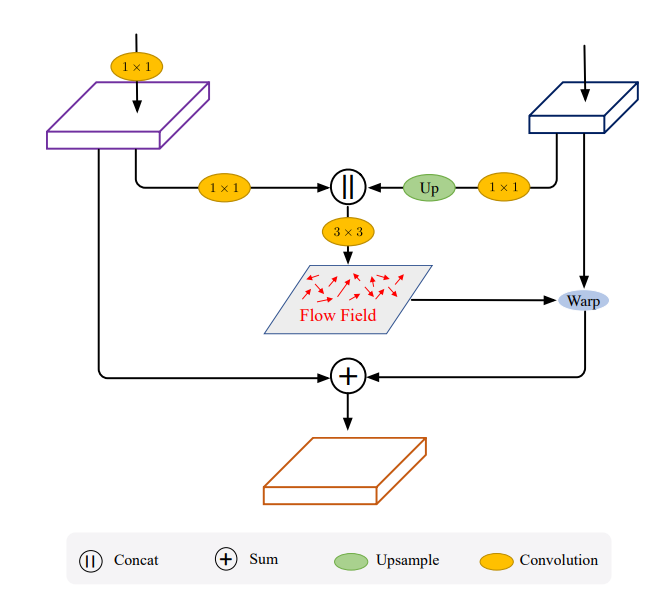
\includegraphics[width=9cm]{sf.png}
    \caption{SF-net\cite{ref34}中的流对齐模块(FAM)}
\centering
\end{figure}
有些工作在改进模块的同时,对编码器-解码器结构进行了设计,如级联了多个编码器-解码器结构的\textbf{shelfnet}\cite{ref23}、将图片金字塔输入共享编码器并行计算的\textbf{swiftnetRN}\cite{ref24}和回归简单编码器-解码器结构并使用多尺度头的\textbf{FFNet}\cite{ref25}等。

\paragraph{引入注意力机制和Transformer块}
注意力机制作为一种非局部方法,具有全局感受野,在建模全局相关性上很有效,已经在语义分割领域广泛使用。一些实时语义分割的工作创新了计算注意力的方法,降低其复杂度,提出了一些非局部模块。

\textbf{DFANet}\cite{ref26}编码器包括三个轻量级Xception分支,每个块输出与下一个分支的相应块的输出连接,并在每个分支的最后加入一个FC注意力模块,计算全局特征并对原特征图加权。
\textbf{FANet}\cite{ref27}提出了快速注意力(FA),在编码器和解码器之间插入FA模块提取全局上下文。FA将自注意力计算中的softmax替换为L2归一化,这本身更高效,并且通过更改矩阵乘法的顺序进一步提高效率。
\textbf{PP-liteseg}\cite{ref28}提出了一个特征融合模块UAFM(Unified Attention Fusion Module),用于解码时融合下采样特征图。UAFM通过空间注意力和通道注意力加权上下采样的特征图,得到输出。

\begin{figure}[!h]
    \centering
    \subfigure[]{
    \begin{minipage}[t]{0.5\linewidth}
    \centering
    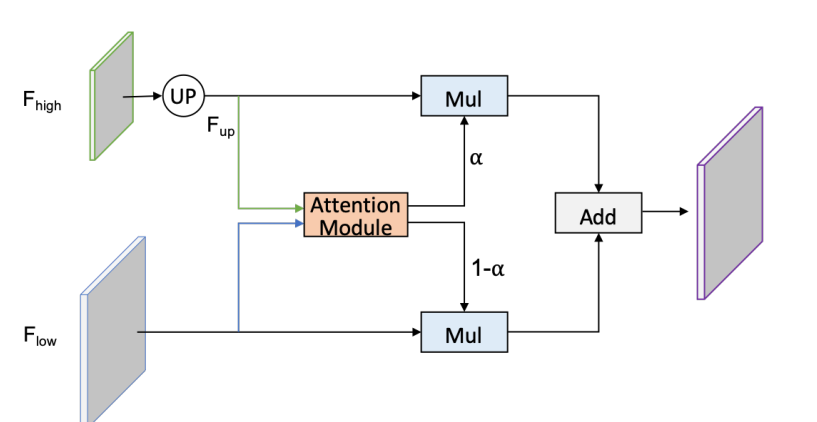
\includegraphics[width=8cm]{pp.png}
    %\caption{fig1}
    \end{minipage}%
    }%
    \subfigure[]{
    \begin{minipage}[t]{0.5\linewidth}
    \centering
    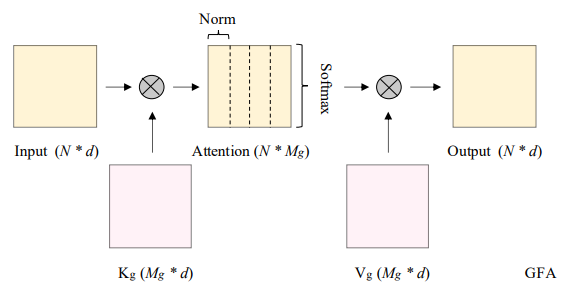
\includegraphics[width=8cm]{rt.png}
    %\caption{fig2}
    \end{minipage}%
    }%

    \subfigure[]{
    \begin{minipage}[t]{\linewidth}
    \centering
    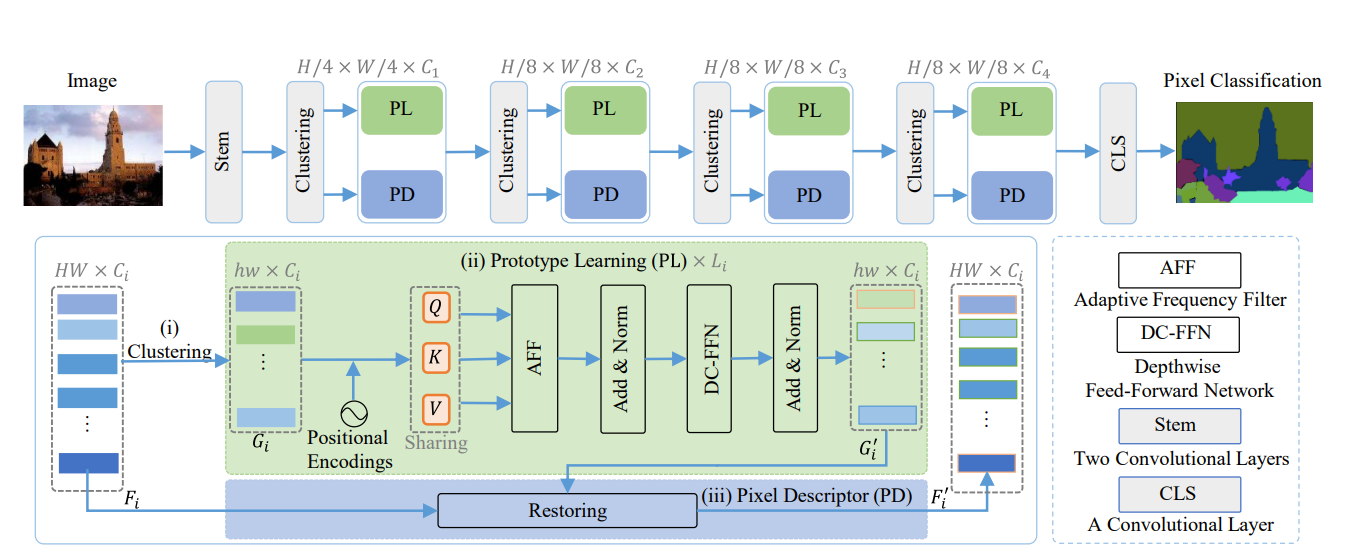
\includegraphics[width=0.9\linewidth]{aff.png}
    %\caption{fig2}
    \end{minipage}
    }%
    \centering
    \caption{(a)PP-liteseg\cite{ref28}中的特征融合模块;(b)RTFormer\cite{ref30}中的GPU友好注意力(GFA);(c)AFFormer\cite{aff}}
\end{figure}
Vision Transformers已经在大量视觉任务中显示出相当强大的结果。但是,尽管取得了成功,基于自注意力机制的Transformer 架构需要强大的计算资源,这超出了许多移动和嵌入式设备的能力。近两年,出现了许多简化Transformer块以适应实时语义分割的工作,取得了很好的效果。

\textbf{TopFormer}\cite{ref29}用Transformer块连接编码器和解码器,先使用级联的mobilenet块生成层次特征图,下采样到统一尺寸后连接作为Transformer块的输入。既融合了多尺度特征,又大大减少了输入的数量,减小了开销。
\textbf{RTFormer}\cite{ref30}改进了自注意力的计算,借鉴了EA(外部注意力)提出GFA(GPU友好注意力),实现线性复杂
度;还提出一个跨分辨率注意力模块,实现了一个高效双分辨率网络。
\textbf{AFFormer}\cite{aff}利用聚类提取原型特征,用Transformer块对原型特征进行特征提取再恢复到原尺寸,因此可以保持一个较高分辨率的特征图,省去了解码器。并且从频率的角度解释自注意力,使用AFF(Adaptive Frequency Filter)计算自注意力,实现线性Transformers,和聚类降维一起提高了效率,实验效果特别好。

\subsubsection{多分支结构}
语义信息和细粒度信息的结合是追求语义分割精度的重要挑战,编码器-解码器结构的方法是通过在下采样提取语义信息,并在上采样过程中恢复细节信息。而实时分割领域还有另一种主流方法,即多分支结构,旨在通过多个分支独立提取不同尺度的特征来解决这个问题。

\textbf{ICNet}\cite{ref31}包括三个独立编码器分支,分别输入尺寸不同的图像。低分辨率分支使用较深的完整网络提取语义信息,中高分辨率分支利用简单的轻量级架构来提取更细粒度的信息以细化输出边界,大大减小参数量,最终用级联特征融合单元融合不同层次的特征。
\textbf{ContextNet}\cite{ref32}利用两个分支有效地提取空间和上下文特征,上下文分支输入分辨率较小的图片,相对较深,空间分支输入高分辨率图片,保留丰富的空间特征。

\textbf{BiSeNet}\cite{ref6}提出了一种经典的双分支架构,由上下文路径和空间分支组成,如图 8 所示。空间路径非常简单,仅使用三个跨步卷积块,而上下文路径基于 Xception 主干快速下采样,扩大感受野,获得较低分辨率的含丰富语义特征的特征图。并设计了注意力细化模块(ARM) 应用于上下文分支的最后两个阶段的输出,使用全局平均池化生成编码全局上下文的特征向量,然后重新加权特征图,两个AFM模块的输出通过特征融合模块(FFM)与空间分支的输出连接在一起。
\textbf{BiSeNet V2}\cite{ref33}沿用了Bisenet v1的设计,本文改进了语上下文路径的模块,并用双边引导聚合层取代FFM,将两个分支的特征按不同层次分别聚合,得到更好的表征。
\begin{figure}[!h]
    \centering
    \subfigure[]{
    \begin{minipage}[t]{0.5\linewidth}
    \centering
    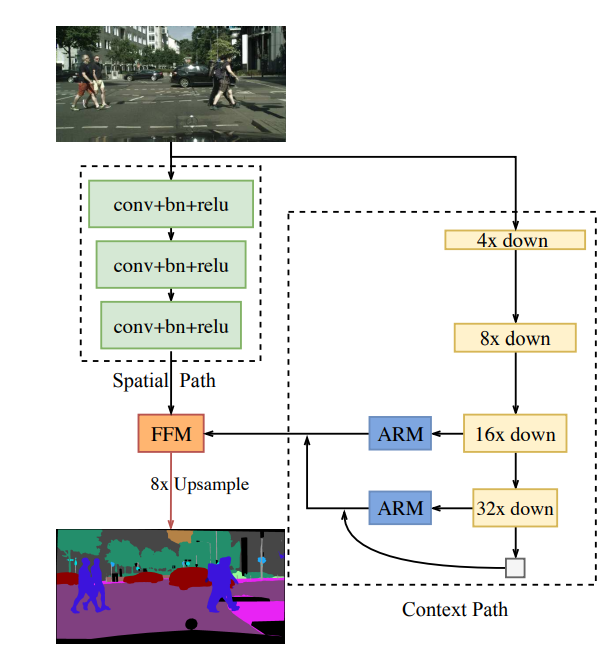
\includegraphics[width=6cm]{bis.png}
    %\caption{fig1}
    \end{minipage}%
    }%
    \subfigure[]{
    \begin{minipage}[t]{0.5\linewidth}
    \centering
    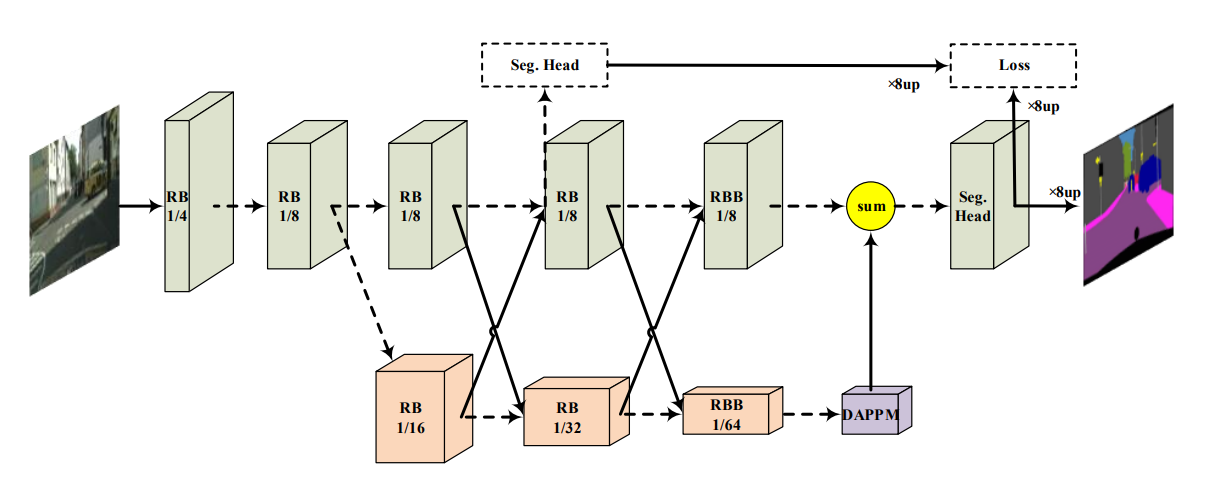
\includegraphics[width=9cm]{ddr.png}
    %\caption{fig2}
    \end{minipage}
    }%
    \centering
    \caption{(a)BiSeNet\cite{ref6};(b)DDRNet\cite{ref39}}
\end{figure}


\textbf{Fast-SCNN}\cite{ref38}让双分支结构共享前几层下采样,优化了冗余,是一种非常轻量级的架构,能够以极高的帧率提供良好的分割结果。\textbf{DDRnet}\cite{ref39}优化了双分支结构,除了共享前几层下采样,还精心设计了双边信息融合模块,两个分支进行了多次信息融
合,并且提出了一个新的上下文模块DASPP,可以捕捉多尺度且扩大有效感受野。

\textbf{STDC}\cite{ref40}设计了一个新的STDC块。它由级联的卷积块组成,在这个过程中获得不同尺度的感受野,并且维度不
断降低(因为语义信息更集中),最终将不同卷积块的特征图连接起来。其中卷积块的数量对参数的影响很小,通过
STDC块,我们可以得到多尺度的特征,并可以通过改变block数量获得可扩展的感受野。通过级联STDC块作为双分支网络的主干,共享两个分支的前几层,提出STDC网络,在训练时还加入了细节分支作为辅助任务。这是一个在实时分割任务上表现很好的的主干网络,被很多后来的工作采用。

\begin{figure}[H]
    \centering
    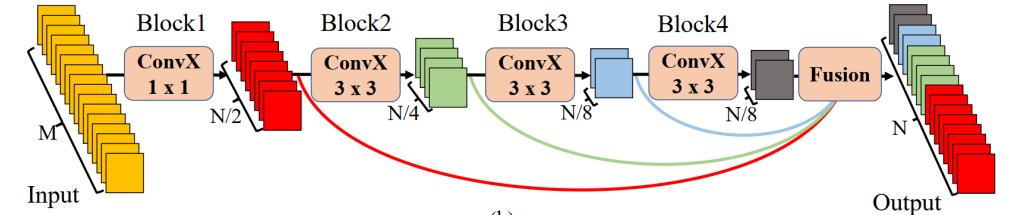
\includegraphics[width=11cm]{stdc.png}
    \centering
    \caption{STDC\cite{ref40}中的STDC块}
\end{figure}
\textbf{PIDNet}\cite{ref41}从传统控制理论出发,认为整个语义分割网络相当于一个PID控制器,其中空间路径保持输入的大部分细节而相当于P分支,上下文路径不断聚合特征而相当于I分支。双分支结构在特征融合时可能因语义信息层次不同而损失表征能力,本文将其解释为PI控制器可能产生的“超调”现象,并引入边界路径作为D分支来抑制超调,
用边界分支指导空间和上下文分支的特征融合,从而提出了一个三分支网络PIDNet。PIDNet认为DDRNet中的DAPPM模块太复杂而不能很好的并行,并且超过轻量级模型的表征能力,设计了简化的PAPPM。借鉴DDRNet的思想,设计了单独的模块Pag,Bag进行三个分支之间的多次信息融合。为了增强模型对边界的敏感性,提高每个分支提取信息的能力,PIDNet在训练时使用了多个辅助任务。
\begin{figure}[!h]
    \centering
    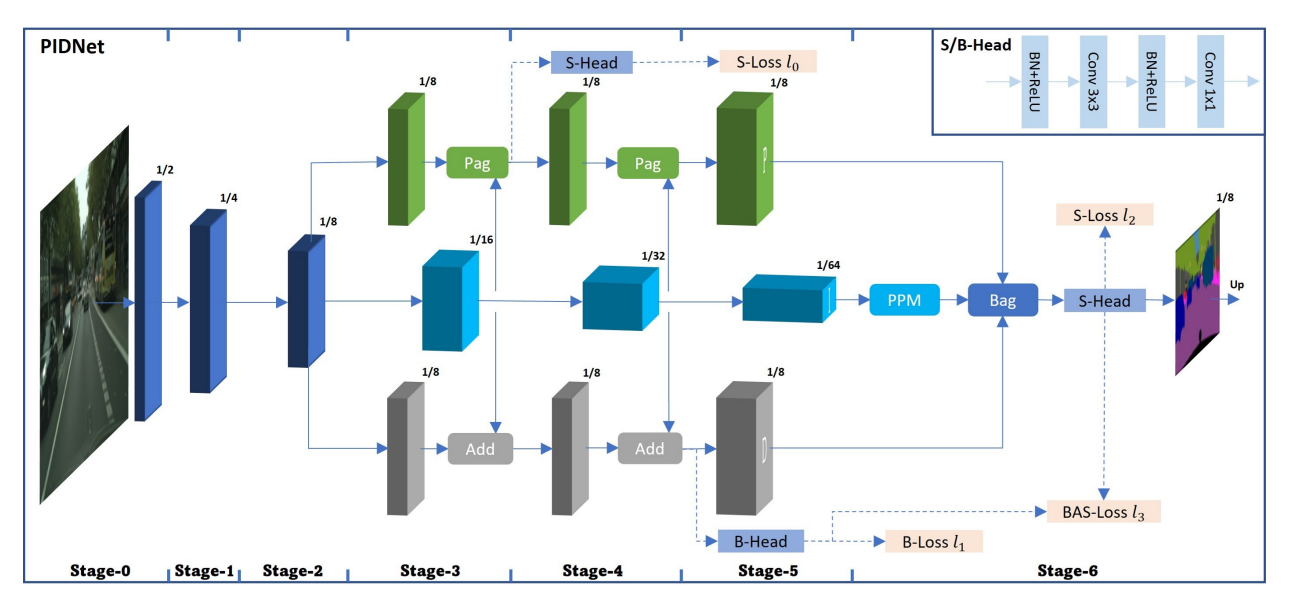
\includegraphics[width=11cm]{pid.png}
\centering
\caption{PIDNet\cite{ref41}}
\end{figure}

\textbf{SeaFormer}\cite{sea}使用提出的Sea注意力改进Transformer块,并将改进后的Sea块加入双分支结构中的上下文路径,大大提高了精度。Sea(squeeze-enhanced Axialattention)注意力简化了自注意力的计算,将特征图按不同维度压缩,再计算压缩后的自注意力,将计算复杂度降到O(HW),与特征图大小呈线性。
\textbf{StrideFormer}\cite{ppl}是百度在2023年4月刚发表的工作,使用了跨步Sea注意力,结合设计的聚合注意力模块 (AAM) 和有效插值模块(VIM)达到了多个数据集上的sota。
\begin{figure}[!h]
    \centering
    \subfigure[]{
    \begin{minipage}[t]{0.9\linewidth}
    \centering
    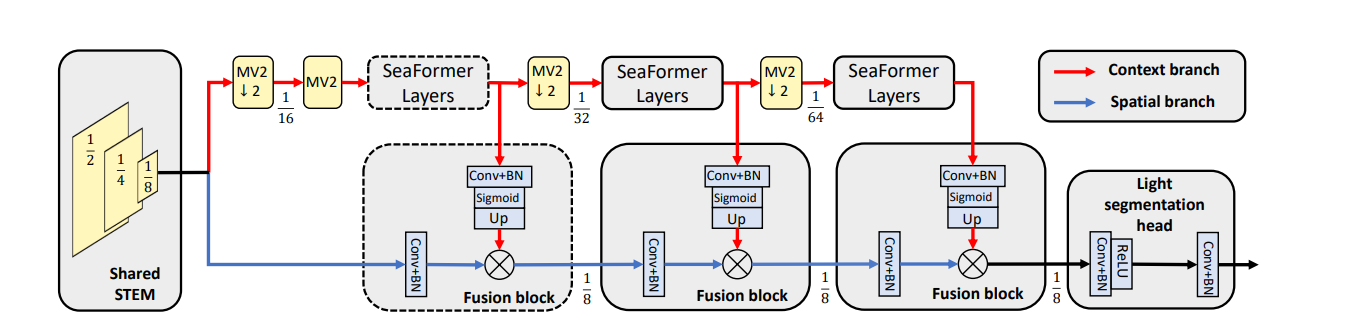
\includegraphics[width=11cm]{sea1.png}
    %\caption{fig1}
    \end{minipage}%
    }%
    
    \subfigure[]{
    \begin{minipage}[t]{0.9\linewidth}
    \centering
    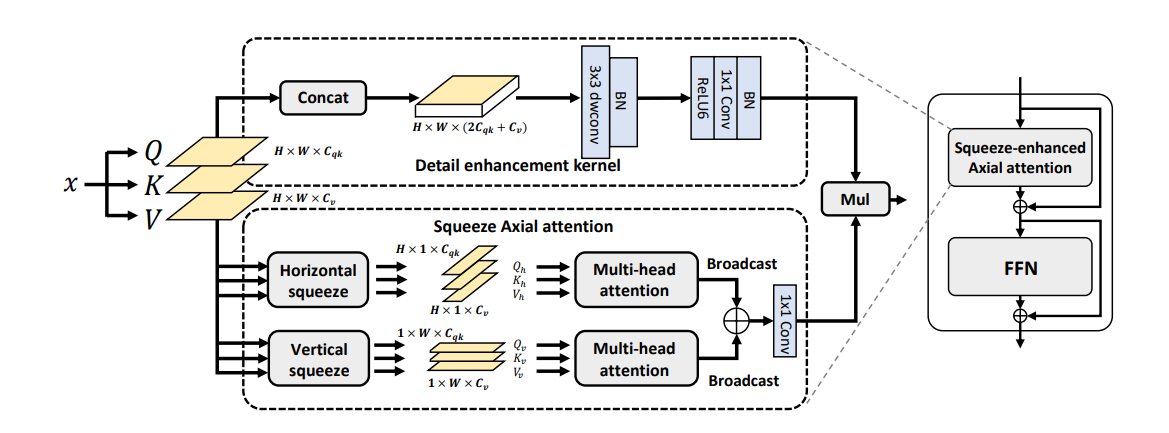
\includegraphics[width=11cm]{sea2.png}
    %\caption{fig2}
    \end{minipage}
    }%
    \centering
    \caption{(a)SeaFormer\cite{sea};(b)Sea Attention}
\end{figure}
\subsection{人像分割}
人像分割一般被认为是语义分割的一个子问题,而它在下列三个方面不同于传统的分割。

\textit{i)人像分割是一个二元分割问题,前景对象仅为人,提供额外的先验信息;}

\textit{ii)人像分割对边界的精度要求更高,并且需要适应复杂的光照条件;}

\textit{iii)结合具体应用场景,人像分割通常仅作为实际应用中的几个步骤之一使用,由于其中许多应用程序在移动设备上运行,分割模型需要轻量级以确保实时速度。}

\textbf{PortraitFCN+}\cite{por+}构建了人像数据集,并提出了基于FCN的人像分割模型。

\textbf{PortraitNet}\cite{porn}是基于mobilenet v2的encoder-decoder网络,并针对人像分割加入两个辅助损失,实现实时人像检测的精度和效率平衡。第一个辅助损失为边界损失,网络在解码器最后一层特征图后,加了一个边界的预测头,从而使分割对边界更敏感;第二个辅助损失为一致约束损失,将原图片A和经过纹理增强(改变亮度、对比度、锐度,加入随机噪声等)的A'都输入网
络,并分别预测。此时认为A的预测结果为更精细的分割,从而使用KL散度损失约束A'向A靠拢,这可以增强网络对复杂光照环境的鲁棒性。
\begin{figure}[H]
    \centering
    \subfigure[]{
    \begin{minipage}[t]{0.5\linewidth}
    \centering
    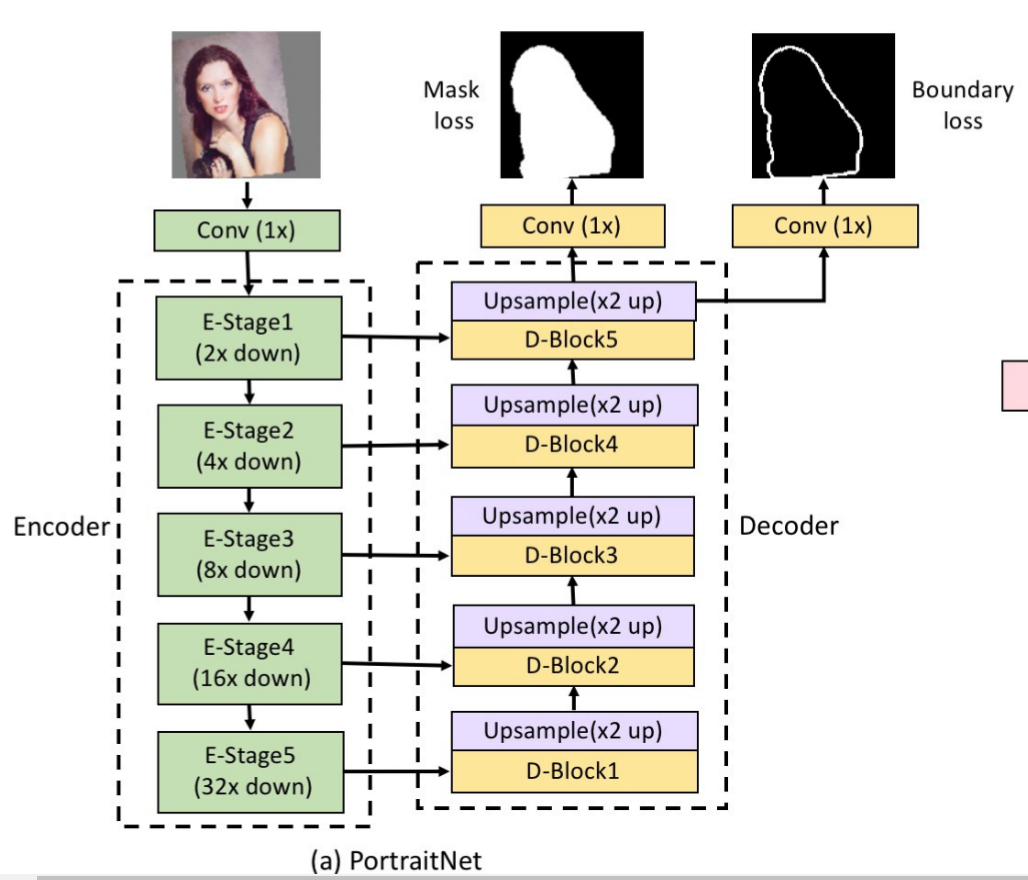
\includegraphics[width=6cm]{p1.png}
    %\caption{fig1}
    \end{minipage}%
    }%
    \subfigure[]{
    \begin{minipage}[t]{0.5\linewidth}
    \centering
    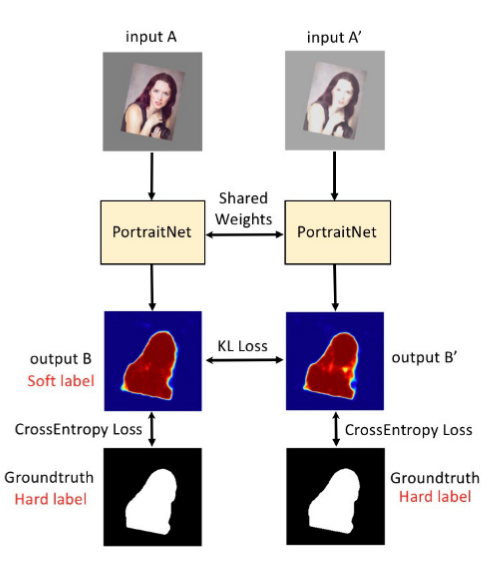
\includegraphics[width=4cm]{p2.png}
    %\caption{fig2}
    \end{minipage}%
    }%
    \centering
    \caption{(a)PortraitNet\cite{porn};(b)PortraitNet中的一致约束损失}
\end{figure}
\textbf{BSN}\cite{bou}主干网络使用Resnet和deeplab v2,引入了边界敏感内核来增强语义边界形状信息。\textbf{Sinet}\cite{ref43}创新了两个上下文模块,并加入了边界的辅助损失,相比Portraitnet大大降低了参数量,且精度损失较小。

\textbf{PP-HumanSeg}\cite{ref42}提出了一个超轻量级的人像分割模型ConnectNet,用极少的参数(0.13M)实现了很强的效果,关键是设计了一种新的连通性损失,实现自监督连接感知学习,让模型自我学习连通性。
\begin{figure}[H]
    \centering
    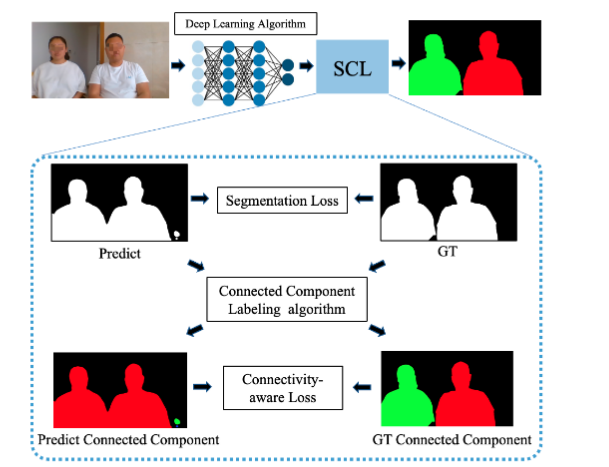
\includegraphics[width=9cm]{pph.png}
\centering
\caption{PP-HumanSeg\cite{ref42}中的自监督连接感知学习(SCL)}
\end{figure}
\section{方案}
在这一部分,我们首先将介绍提出的人像分割模型。它采用了非对称编码器-解码器结构,包括由反转残差块组成的编码器、多尺度上下文模块和由特征融合模块组成的轻量解码器。
接着,我们将详细解释精心设计的后处理模块,可以实现效果更自然的虚拟背景替换。最后,我们将给出整个网络的结构和使用的部分优化方法。
\subsection{反转残差块}
MobileNetV3\cite{ref12}具有强大的特征提取能力,是经典的轻量级卷积神经网络,具有优秀的精度-速度平衡,常作为主干网络被应用到实时分割模型中。
我们根据MobileNetV3给出的高效反转卷积块,设计了主干网络,作为编码器提取并聚合输入图片的语义特征。

\paragraph{内部结构}反转残差块的结构如图\ref{fig:1}所示。输入特征先经过一个扩张卷积。这是一个标准的1*1卷积块,包括激活函数和归一化层,它会将输入特征的维度扩大,以增强特征提取能力,在更高的维度提取特征.
扩张后的特征图将通过一个3*3逐深度卷积块和一个1*1逐点卷积块,前者可以扩大感受野,捕捉每张特征图的局部特征,后者将聚合通道间的特征。
当且仅当输入与输出通道数相等时,残差连接将输入与最后一个卷积块的输出相加。
\begin{figure}[!h]
  \centering
  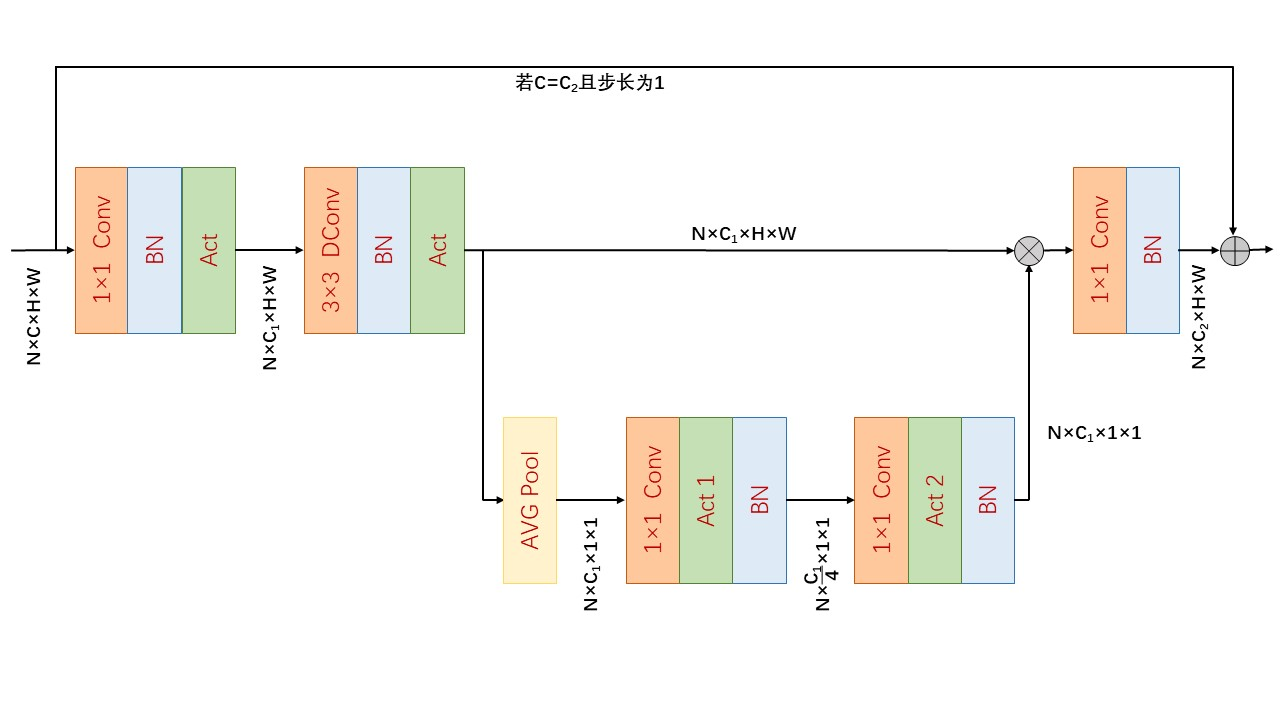
\includegraphics[width=12cm]{res.png}

  \centering
  \caption{反转残差块}
  \label{fig:1}
\end{figure}

其中,深度分离卷积大大降低了参数量,提高了计算效率。
假设输入的特征图尺寸为$N*C_1*H*W$,输出维度为$C_2$。经过分析可得,3*3标准卷积层的参数量为$9C_1C_2$,计算量(仅考虑卷积运算中的乘法)为$9HWC_1C_2$;3*3深度分离卷积层的参数量为$9C_1+C_1C_2$,计算量为$9HWC_1+HWC_1C_2$,二者降低了$\frac1{C_2}+\frac19$。
由于扩张卷积块会提高输入特征的维度,$C_1$往往是C和$C_2$的3-6倍,深度分离卷积降低计算量的效果很明显。
\paragraph{线性瓶颈层}由MobileNetV2\cite{ref11},若将特征空间中信息的分布视为兴趣流形,那么非线性层会破坏流形的分布,使信息丢失。经过分析易知,当兴趣流形处于特征空间的低维子空间,即特征空间维度较高时,由于其他维度的特征大概率可以恢复被破坏的信息,此时非线性层可以保留信息,同时引入函数的复杂性。
而当特征空间维度较低时,非线性层造成的破坏可能无法恢复。因此,反转残差块的第二个降维的逐点卷积使用了线性瓶颈层,没有连接激活函数。


\paragraph{SE}
由SENet\cite{se},squeeze-and-excite模块作为一种轻量注意力模块,可以根据全局信息自适应地加权不同通道的特征图。输入特征先经过全局平均池化层,得到每个特征图的均值作为全新信息表征,再经过两个全连接层(1*1卷积层)合并通道间的信息,最终得到每张特征图的加权值。
这两个全连接层后常接非线性层,将在下一部分详细讲述。


\paragraph{非线性层}
由MobileNetV3,激活函数hwish()可以有效提高精度,其表达式为
\[hwish(x)=x\sigma(x)\]
但是,sigmoid函数需要计算指数,复杂度较高,\cite{ref12}将其简化为$\frac{ReLU6(x+3)}6$,实验显示精度影响不大。其中,
\[ReLU6(x) = 
\begin{cases}
    0, & \text{if } x < 0 \\
    x, & \text{if } 0 \leq x \geq 6 \\
    0, & \text{if } x  >6
\end{cases}\]
同时,hwish函数被简化为反转残差块中应用的h-swish函数
\[hswish(x)=x\frac{ReLU6(x+3)}6\]

如图\ref{fig:1}所示,反转残差块中的Act()会根据所处阶段,选择ReLU或h-swish作为激活函数。

SE模块中的Act1()使用ReLU函数,Act2使用简化的sigmoid函数,将激活值约束到[0,1]。

\subsection{简化聚合金字塔池化模块(SAPPM)}
如图\ref{fig:2}所示,我们提出了一个简化聚合金字塔池化模块(Simple Aggregation PPM, SAPPM),可以提取并聚合多尺度的上下文特征。
它首先利用金字塔池化模块捕捉多尺度地输入特征,金字塔池化模块有4个平均池化操作,池化网格尺寸分别为1*1,2*2,3*3和6*6。
不同尺寸的输出特征分别输入1*1卷积块,来产生细化的特征,并上采样到与原图同一大小。
同时,经1*1卷积块提取的特征将与每个尺寸提取的上下文特征平行相加合并,得到不同尺寸的融合特征。最后,经过两次沿维度连接和残差连接,使用卷积块提取聚合特征,得到最终输出。
\begin{figure}[!h]
  \centering
  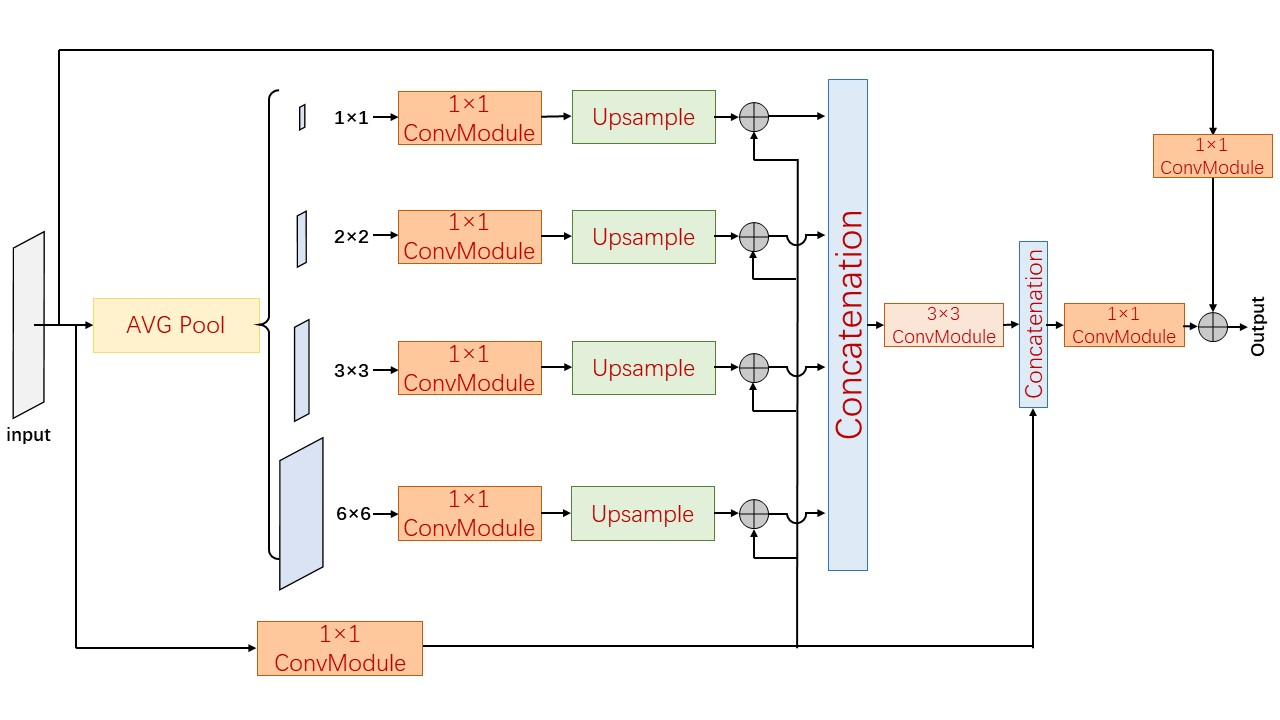
\includegraphics[width=12cm]{sappm.png}

  \centering
  \caption{简化聚合金字塔池化模块(SAPPM)}
  \label{fig:2}
\end{figure}

与原始PPM和SPPM相比,我们的SAPPM多次聚合上下文特征,具有更强的提取和表征能力。
与DDRNet中的DAPPM(Deep Aggregation PPM)和PIDNet中的PAPPM(Parallel Aggregation PPM)相比,我们简化了聚合过程,去除了冗余连接,并且将跨步大卷积核池化简化为固定池化尺寸,减轻了对超参数的依赖(由9个简化为3个)。
实验结果表明,我们的SAPPM实现了最佳的效果。


\subsection{流对齐-注意力融合模块}

\subsubsection{设计动机}
\paragraph{语义流对齐}
大部分基于编码器-解码器的语义分割模型,都会在解码器对高语义、低分辨率的特征图进行上采样,同时利用下采样阶段的高分辨率、低语义的特征图指导上采样并融合细节信息。
但是,这两部分特征图在语义层次存在差距,我们认为,由于语义信息无法很好地对齐,特征融合时会引起语义的无效传播。
SFNet\cite{ref34},受到光流的启发,提出了“语义流”的概念。光流广泛用于视频处理任务,以表示视觉场景中由相对运动引起的物体、表面和边缘的明显运动模式。
而来自同一图像的任意分辨率的两个特征图之间的关系,也可以用每个像素从一个特征图到另一个特征图的“运动”来表示。
我们可以明确学习不同分辨率的两个网络层之间的语义流,通过流对齐模块,使用流场对特征图进行修正,从而实现语义的对齐,更加有效地融合不同分辨率的信息。

\paragraph{轻量解码器}
我们的解码器仅保留了一个阶段,包括流对齐-注意力融合模块,大大提高了计算效率。我们主要出于以下两点考虑:
\textit{i)人像分割是一个二元分割问题,并且前景对象仅为人,人占据了图片的一个较大的连通域,是一个比较简单的任务,不需要冗余的细节特征。}
\textit{ii)我们的多尺度上下文模块具有强大的特征提取能力,流对齐注意力融合模块可以高效融合不同分辨率特征图中的信息。}

\subsubsection{模块细节}
为了对齐不同分辨率特征图的语义层次,使信息在融合时有效传播,我们设计了流对齐-注意力融合模块,包括流对齐模块和统一注意力模块,其结构如图\ref{fig:3}所示。
\begin{figure}[!h]
  \centering
  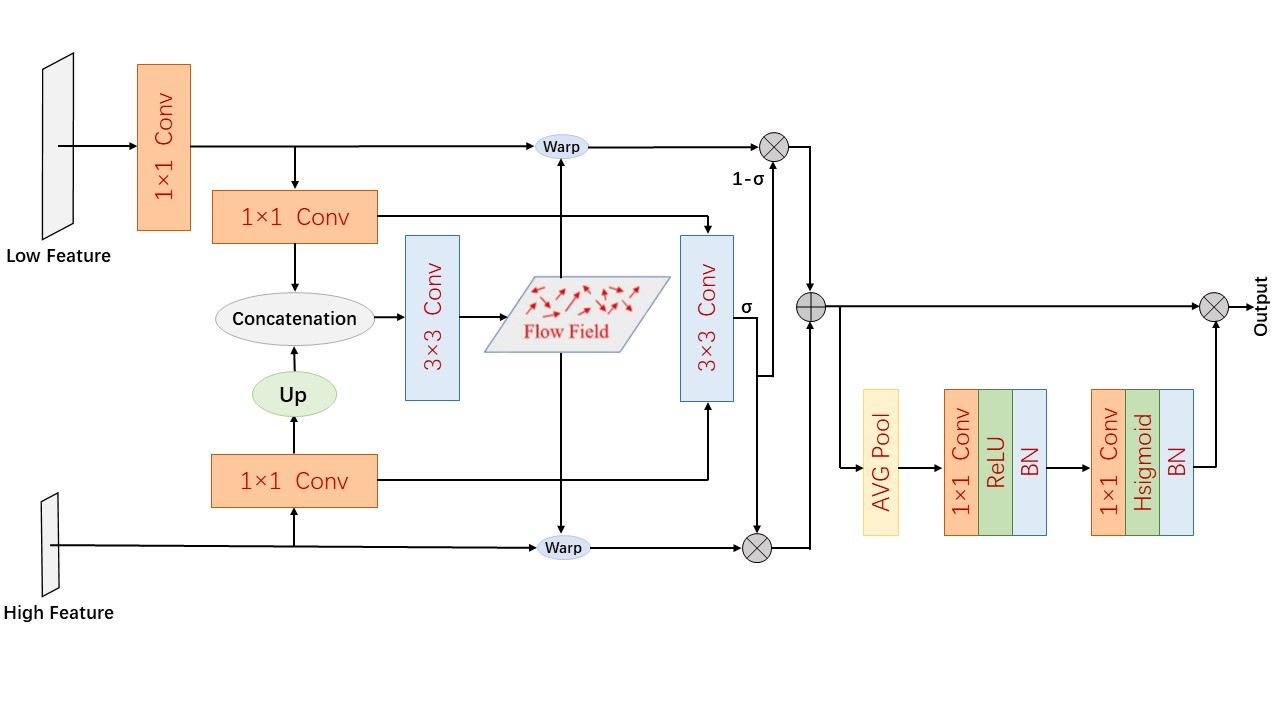
\includegraphics[width=12cm]{cusfuse.png}

  \centering
  \caption{流对齐-注意力融合模块}
  \label{fig:3}
\end{figure}
\paragraph{流对齐模块}
我们采用了SFNet中的流对齐方法。令输入为不同分辨率的特征图$F_l$和$F_h$,其中$F_l$为分辨率高、语义信息低的特征图。
首先特征图分别经过1*1卷积层,得到$F_{el},F_{eh}$,将$F_{eh}$经双线性上采样后,与$F_l$沿维度连接起来,输入一个3*3卷积层。
这个3*3卷积层将提取特征图之间的语义流场,流场维度为4,分别包含$F_h$和$F_l$的流场偏移(x和y两个维度)。
我们将利用这个偏移量分别修正细化两部分特征图,如图\ref{fig:4}所示。流场偏移量将作用于双线性插值的采样网格,从而对特征图扭曲以对齐语义信息。
\begin{figure}[h]
  \centering
  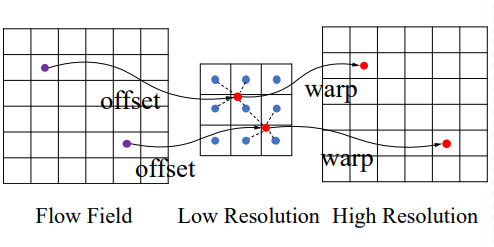
\includegraphics[width=6cm]{1.png}

  \centering
  \caption{warp操作\cite{ref34}}
  \label{fig:4}
\end{figure}

\paragraph{统一注意力模块}

为了使特征更好地融合,我们在统一注意力模块中先计算了逐像素注意力和通道注意力,增强其中重要的部分。

在计算逐像素注意力时,我们希望充分利用高级语义特征,让低级特征作为高级特征的补充。
具体来说,我们将$F_{el},F_{eh}$输入一个3*3卷积层,并经过sigmoid非线性层,得到与特征图大小相等的权重图,从而通过逐像素点加权,强调特征图中的重要部分。
我们使用了共享权重图,使用原始权重$\sigma$与高语义特征图相乘,并使用$1-\sigma$与高分辨率特征图相乘,通过这种方式,可以让$\sigma$更好的表征特征图的共同信息。

我们使用了SE模块计算通道注意力,计算每个通道的加权值。

\subsection{后处理模块}
\subsubsection{图像的后处理操作}
\textbf{膨胀操作}

膨胀是将图像A与核B进行卷积,一般选取正方形的卷积核,对图像的局部求最大值的操作。核B与图形卷积,即计算核B覆盖区域的像素最大值,并把最大值赋值给参考点指定的像素。\textbf{膨胀效果可以使图像中的高亮区域逐渐增长。}

用数学公式表达即为:
\[
dst\left(x,y\right) = max_{\text{$(x',y'):element(x',y')\neq 0$}} src \left(x+x',y+y'\right)      
\]
用$\left(x,y\right)$周边区域$\left(x+x',y+y'\right)$内最大值代替$\left(x,y\right)$的值。



\textbf{腐蚀操作}

腐蚀与膨胀是相反的效果,腐蚀是求局部最小值。\textbf{膨胀效果可以使图像中的高亮区域逐渐收缩。}

用数学公式表达即为:
\[
dst\left(x,y\right) = min_{\text{$(x',y'):element(x',y')\neq 0$}} src \left(x+x',y+y'\right)      
\]
用$\left(x,y\right)$周边区域$\left(x+x',y+y'\right)$内最小值代替$\left(x,y\right)$的值。


\textbf{后处理操作}

后处理操作是对模型输出图片先进行腐蚀操作,然后再进行膨胀操作。这种组合操作的主要目的是在保持对象形状的同时,减少噪声和小的细节。

效果对比图如下:
\begin{figure}[!h]
    \centering
    \subfigure[]{
    \begin{minipage}[t]{0.4\linewidth}
    \centering
    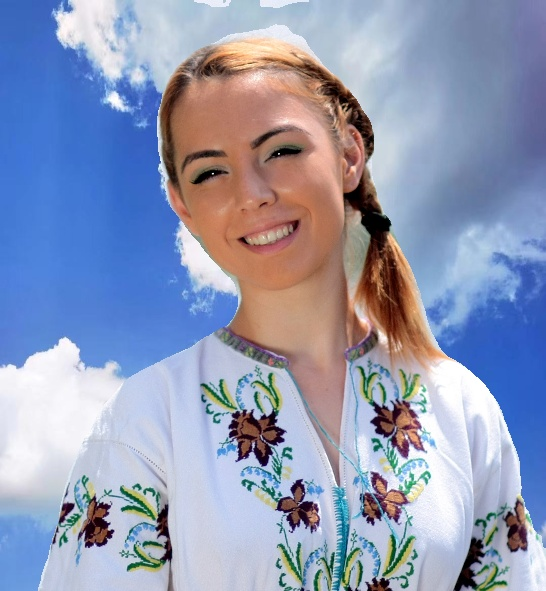
\includegraphics[width=5cm]{output_result1.jpg}
    %\caption{fig1}
    \end{minipage}%
    }%
    \subfigure[]{
    \begin{minipage}[t]{0.4\linewidth}
    \centering
    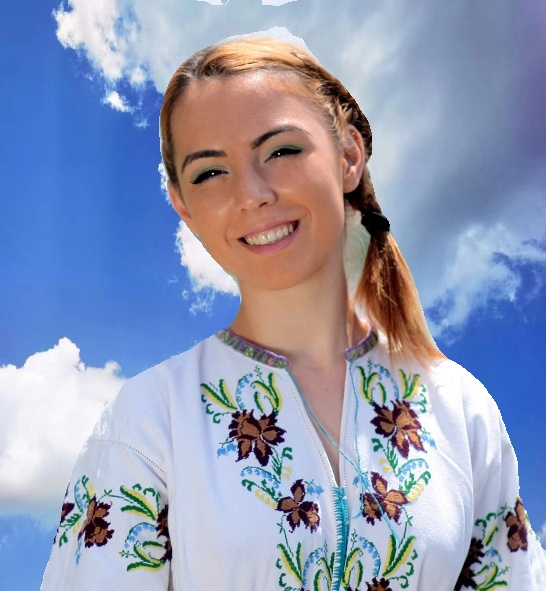
\includegraphics[width=5cm]{output_erode.jpg}
    %\caption{fig2}
    \end{minipage}%
    }%

    \subfigure[]{
    \begin{minipage}[t]{0.4\linewidth}
    \centering
    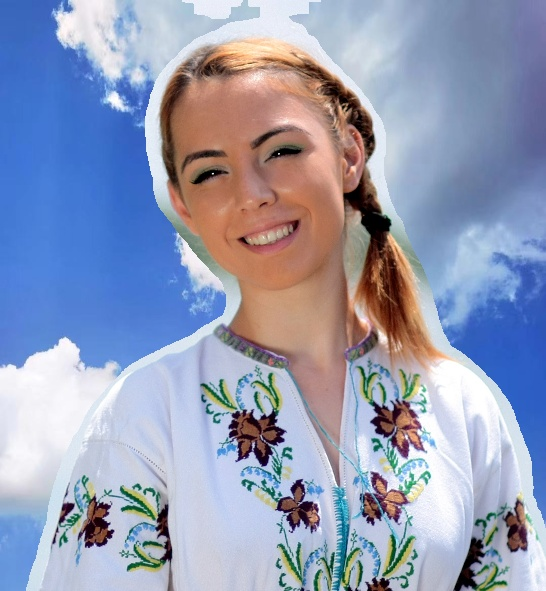
\includegraphics[width = 5cm]{output_dilate.jpg}
    %\caption{fig2}
    \end{minipage}
    }%
    \subfigure[]{
    \begin{minipage}[t]{0.4\linewidth}
    \centering
    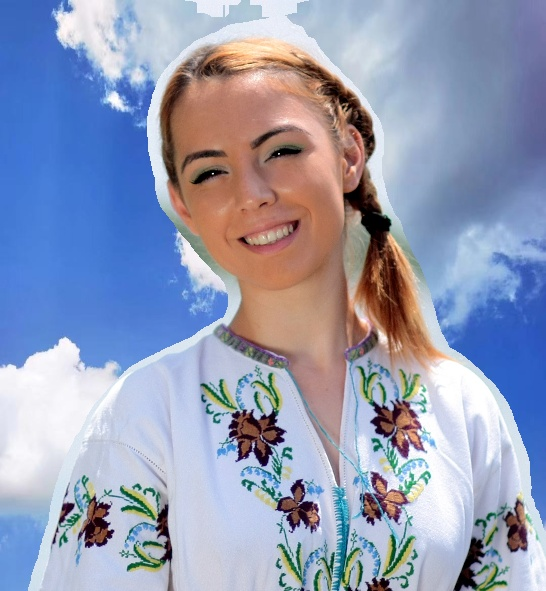
\includegraphics[width=5cm]{output_pro.jpg}
    %\caption{fig2}
    \end{minipage}%
    }%
    \caption{(a)原图;(b)腐蚀操作效果图;(c)膨胀操作效果图;(d)后处理操作效果图}

\end{figure}

\subsubsection{光流法操作}
在一个图像平面上,物体的运动往往是通过图像序列不同图像灰度分布的不同体现的,即光流场(optical flow field)。

光流场是一个二维矢量场,它反映了图像上每一点灰度的变化趋势,可看成是带有灰度的像素点在图像平面上运动而产生的瞬时速度场。它包含的信息即是各像点的瞬时运动速度矢量信息。

\textbf{光流法基本假设}

1.\textbf{亮度恒定不变。}即同一目标在不同帧间运动时,其亮度不会发生改变。这是基本光流法的假定(所有光流法变种都必须满足),用于得到光流法基本方程。

2.\textbf{时间连续或运动是"小运动"。}即时间的变化不会引起目标位置的剧烈变化,相邻帧之间位移要比较小。同样也是光流法不可或缺的假定。

\subsection{基本约束方程}

考虑一个像素I(x,y,t)在第一帧的光强度它移动了 (dx,dy)的距离到下一帧,用了dt时间。因为是同一个像素点,依据上文提到的第一个假设我们认为该像素在运动前后的光强度是不变的,即:
\[
I\left((x,y,t)\right) = I\left(x + dx,y+dy,t+dt\right)    
\]
对右端泰勒展开后去除二阶小量,得:
\[
\frac{\partial I}{\partial x} \frac{\mathrm{d} x}{\mathrm{d} t} +\frac{\partial I}{\partial y} \frac{\mathrm{d} y}{\mathrm{d} t}+\frac{\partial I}{\partial t} \frac{\mathrm{d} t}{\mathrm{d} t}
\]
设u,v分别为光流分别为沿X轴与Y轴的速度矢量,得:
\[
u = \frac{\mathrm{d} x}{\mathrm{d} t} ,v =\frac{\mathrm{d} y}{\mathrm{d} t}   
\]
令$I_x = \frac{\partial I}{\partial x} ,I_y =\frac{\partial I}{\partial Y} ,I_t=\frac{\partial I}{\partial t} $分别表示图像中像素点的灰度沿X,Y,T方向的偏导数

综上,上式可化简为:
\[
I_x u +I_y v+I_t = 0    
\]
其中,Ix,Iy,It均可由图像数据求得,而(u,v)即为所求光流矢量。

而我们使用的DIS(Dense Inverse Search)光流方法是一种基于密集采样的光流方法,属于快速稠密光流,是一种在光流质量和计算时间中取得平衡的算法。优点是运算速度快的稠密光流,可达到实时要求。

\textbf{具体方案}

1.根据时序图像,计算相邻两帧的DIS光流(对应像素的位置关系)

2.根据DIS光流找到前一帧融合结果Flast的运动预测结果P

3.根据光流大小判断融合权重W

4.融合结果 $F = S\times W + P\times \left(1-W\right)$,其中S为当前帧分割结果,P为上一帧的运动预测结果

\textbf{对比光流后处理的分割效果}

\begin{figure}[H]
    \centering
    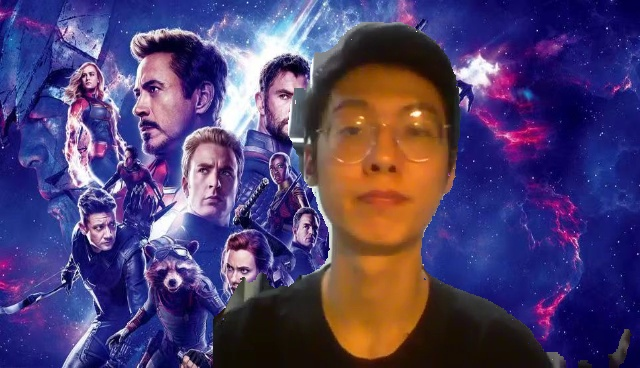
\includegraphics[width = 0.6\textwidth]{output_shuai.jpg}
    \caption{未使用光流法}
    \label{fig:image7}

\end{figure}

\begin{figure}[H]
    \centering
    \begin{minipage}[t]{0.32\textwidth}
        \centering
        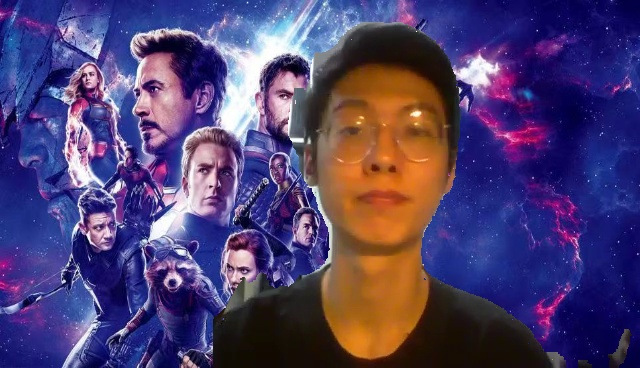
\includegraphics[width=\textwidth]{output_0.jpg}
        \caption{光流法1}
        \label{fig:image8}
    \end{minipage}\hfill
    \begin{minipage}[t]{0.32\textwidth}
        \centering
        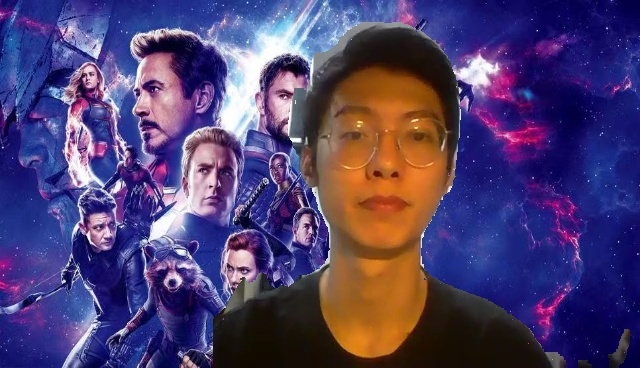
\includegraphics[width=\textwidth]{output_1.jpg}
        \caption{光流法2}
        \label{fig:image9}
    \end{minipage}\hfill
    \begin{minipage}[t]{0.32\textwidth}
        \centering
        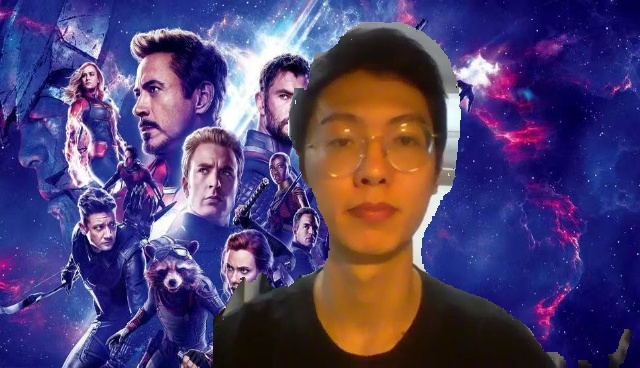
\includegraphics[width=\textwidth]{output_2.jpg}
        \caption{光流法3}
        \label{fig:image10}
    \end{minipage}
\end{figure}
\subsection{网络结构}
我们网络的整体结构如图\ref{fig:net}所示,包括编码器,SAPPM和轻量解码器。


首先,给定一个输入图像,我们的网络利用一个通用的轻量级主干网络作为编码器来提取层次特征。
具体地说,我们的编码器由反转卷积块组成,降低输入图像的分辨率,并聚合提取语义特征,共分四个阶段进行,每个阶段的步长为2,因此最终特征大小为输入图像的1/16。
主干网络的具体设置如下表所示,超参数设置参考了MobileNetV3的前9层,因此,我们在训练时加载了MobileNetV3的参数作为预训练权重。

\begin{table}[!ht]
  \centering
  \begin{tabular}{|l|l|l|l|l|l|l|l|l|}
  \hline
      stage & layer & kernal size & input channels & mid channels & out channels & SE module & activation & stride \\ \hline
      1 & 1 & 3 & 3 & - & 16 & - & ReLU & 2 \\ \hline
      2 & 2 & 3 & 16 & 16 & 16 & √ & ReLU & 2 \\ \hline
      3 & 3 & 3 & 16 & 72 & 24 & ~ & ReLU & 2 \\ \hline
      3 & 4 & 3 & 24 & 88 & 24 & ~ & ReLU & 1 \\ \hline
      4 & 5 & 5 & 24 & 96 & 40 & √ & HSwish & 2 \\ \hline
      4 & 6 & 5 & 40 & 240 & 40 & √ & HSwish & 1 \\ \hline
      4 & 7 & 5 & 40 & 240 & 40 & √ & HSwish & 1 \\ \hline
      4 & 8 & 5 & 40 & 120 & 48 & √ & HSwish & 1 \\ \hline
      4 & 9 & 5 & 48 & 144 & 48 & √ & HSwish & 1 \\ \hline
  \end{tabular}
  \caption{主干网络超参数设置。其中第一层为标准卷积块,其余为反转残差块}
\label{table:1}
\end{table}
其次,我们采用SAPPM对长程依赖关系进行建模。以编码器的输出特征为输入,SAPPM产生一个聚合全局上下文信息的特征。输出的特征具有很好的表征能力并且融合了多尺度信息。

最终,我们采用流对齐-注意力融合模块,聚合SAPPM模块输出的高语义特征与下采样时1/4尺寸特征图的细节特征。先利用流对齐模块指导低分辨率特征图的上采样,统一不同特征图的语义层次;
然后计算像素和通道注意力,加权特征图。该1/4尺寸特征图的维度在分割头中被压缩2(背景和人),再上采样到原尺寸,采用softmax值预测并计算交叉熵损失。

同时,我们使用了一些辅助任务来优化网络的训练,将在下一部分详细说明。
\subsection{训练技巧}
我们在训练时还加入了一些训练技巧,使用了OHEM采样方式,深监督和边界损失,实验表明,这些技巧对效果的提升很明显。
\paragraph{OHEM}在线难样本挖掘(OHEM,Online Hard Example Mining),使用特殊的采样方式解决类别不均衡问题。
具体来说,在训练时,只有置信分数在0.9以下的像素值点会被拿来训练,至少要保留131072个像素值点,从而可以让模型针对“难点”训练。

\paragraph{深监督}深监督已经在许多工作中印证了其有效性,但是由于我们的模型网络较浅,仅使用了一个辅助分割头,并测试了放在不同位置对精度的影响。
具体来说,除了在解码器的顶端使用分割头进行预测,我们还在编码器的第四阶段结束时加入一个辅助分割头,将第三阶段的特征图输入两个3*3卷积块后使用1*1卷积层得到预测,并计算损失。
该辅助损失的权重为0.4,在预测时会被忽略。

\paragraph{边界损失}
我们希望模型对边界敏感,学习到与边界相关的统计规律。因此,我们在编码器的第三阶段结束时,插入了边界分支。该分支包块两个3*3标准卷积块,并使用1*1卷积层预测边界,将边界预测与我们从GT分割图中生成的GT边界图比较,计算二元加权交叉熵损失。

我们模型的总体损失函数为
\[L=\alpha L_{seg} + \beta L_{aux-seg}+\theta L_{boundary}\]

其中$L_{seg}$为解码器顶端的分割头预测的交叉熵损失,$L_{aux-seg}$为深监督的辅助损失,$L_{boundary}$为边界分支的损失。在最终模型中,权重$\alpha=1.0, \beta=0.4,\theta=2.0$。
\section{实验与优化过程}
\textit{我们的实验均基于mmSegmentation2.0,设置了固定的随机种子304,并在提交的源代码中提供了全部的配置文件、模块代码和训练日志,结果均可查、可复现。}
\subsection{优化思路}
受到人像分割的一些经典工作启发\cite{porn,ref42,ref43},我们决定采用编码器-解码器结构构建我们的模型。
同时,我们对比了大量基于编码器-解码器结构的语义分割工作,将整个模型抽象为“编码器(主干网络)+上下文模块(neck)+解码器(特征融合模块)”,并基于此进行优化,如图\ref{fig:5}所示。


我们将“MobileNetV3+PAPPM+sea_fusion”作为我们的基准,其中sea_fusion表示seaformer中的融合模块,以mIoU(平均交并比)作为主要评价指标,aAcc(平均类别精度)和mAcc(平均像素精度)作为辅助评价指标。
\begin{figure}[H]
  \centering
  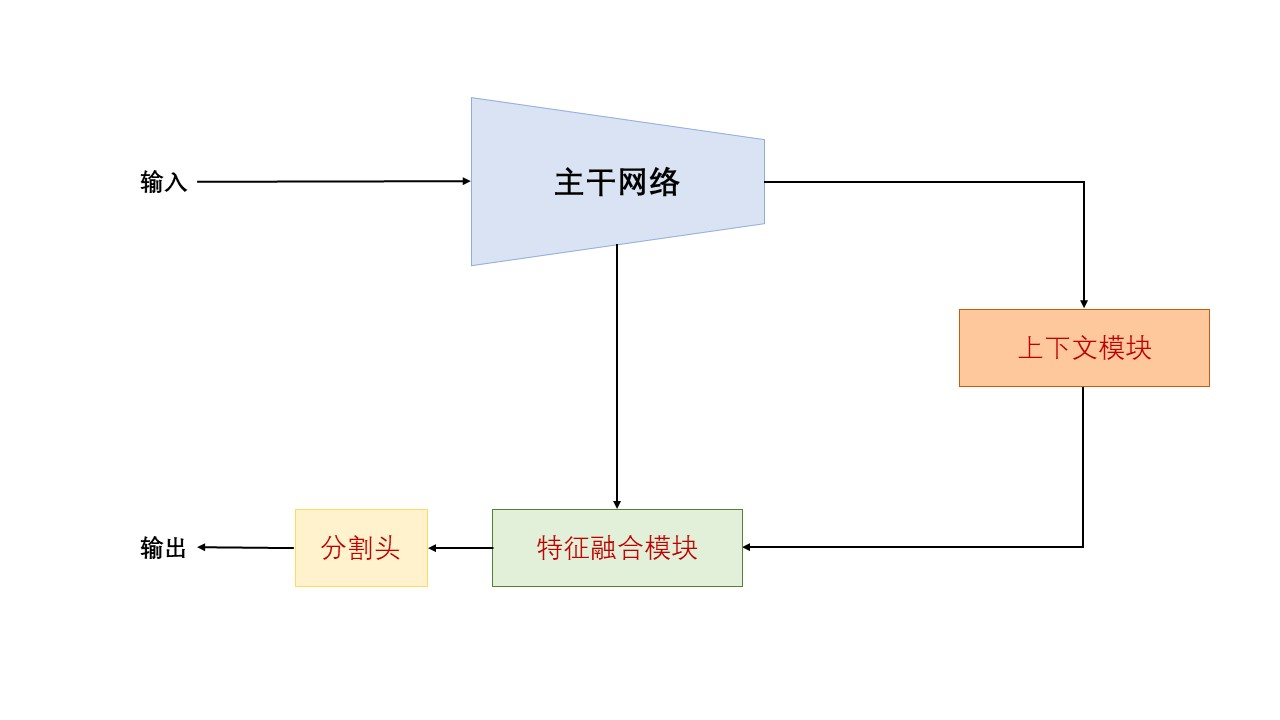
\includegraphics[width=12cm]{ar.jpg}

  \centering
  \caption{模型抽象结构图}
  \label{fig:5}
\end{figure}
对于编码器,为了节省工作量,我们选择成熟的主干网络MobileNetV3作为我们的编码器,而没有自己设计,从而可以使用预训练权重初始化,加快收敛。

对于上下文模块,我们对比了PPM,DAPPM,PAPPM等效果较好的上下文模块,通过设计结构和调整超参数得到SAPPM。

对于特征融合模块,我们做了大量的实验,对比多种现有模块,并对他们的超参数进行调整以适应整体网络,最终结合语义流等思想提出了流对齐-注意力融合模块,有效提升了精度。

我们还使用了多种其他方法来优化我们的模型,如OHEM,增加边界预测的辅助任务和深监督,有效提高了精度。


\subsection{数据集}
我们在Supervise-Portrait数据集上进行实验。
Supervise-Portrait是Portraitnet作者从公开通用人像分割数据集Supervisory.ly\cite{sur}中精心挑选的人像分割数据集,包含高质量的注释,具有复杂的背景和遮挡。
我们在其中删去了大部分标注图只有背景类别的图片(部分标注图疑似错误),并筛去了一些比较奇异的图片,
最终随机选择了1945幅不同尺寸的图像作为训练数据集,243幅图像作为验证/测试数据集。数据集中的一些样例如图\ref{fig:6}所示。
\begin{figure}[!h]
  \centering
  \subfigure[]{
  \begin{minipage}[t]{0.2\linewidth}
  \centering
  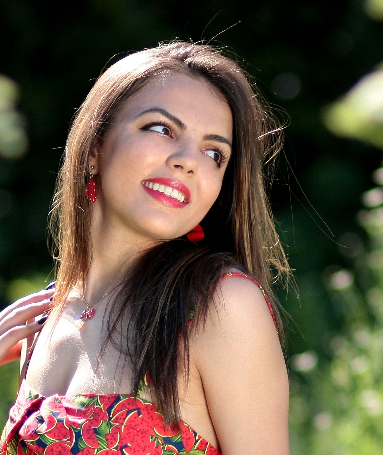
\includegraphics[width=1\linewidth]{1.jpg}
  %\caption{fig1}
  \end{minipage}%
  }%
  \subfigure[]{
  \begin{minipage}[t]{0.2\linewidth}
  \centering
  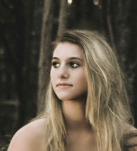
\includegraphics[width=1\linewidth]{2.jpg}
  %\caption{fig2}
  \end{minipage}%
  }%
  \subfigure[]{
  \begin{minipage}[t]{0.2\linewidth}
  \centering
  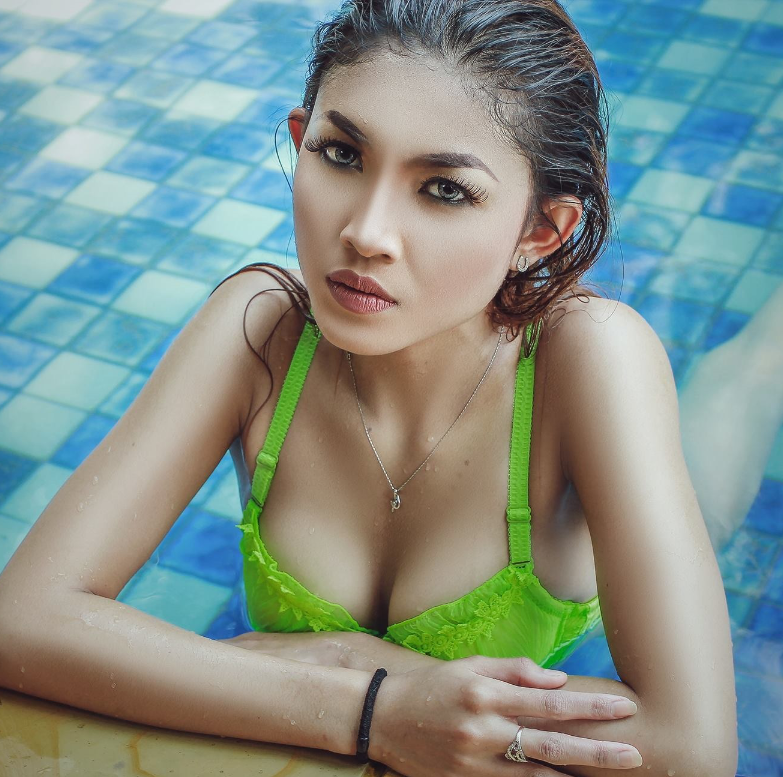
\includegraphics[width=1\linewidth]{3.jpg}
  %\caption{fig2}
  \end{minipage}%
  }%
  \subfigure[]{
  \begin{minipage}[t]{0.2\linewidth}
  \centering
  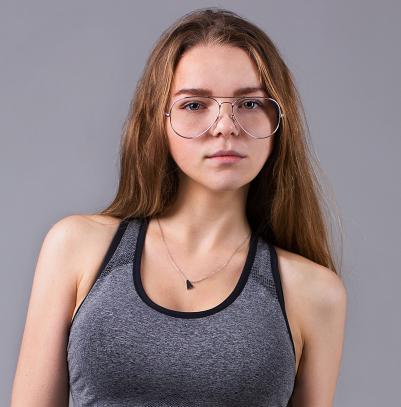
\includegraphics[width=1\linewidth]{4.jpg}
  %\caption{fig2}
  \end{minipage}%
  }%

  \subfigure[]{
  \begin{minipage}[t]{0.2\linewidth}
  \centering
  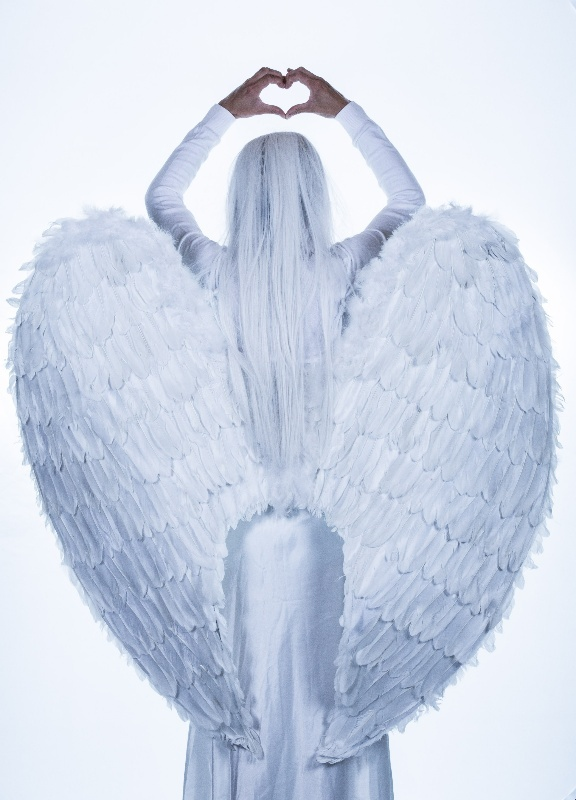
\includegraphics[width=1\linewidth]{5.jpg}
  %\caption{fig2}
  \end{minipage}%
  }%
  \subfigure[]{
  \begin{minipage}[t]{0.2\linewidth}
  \centering
  \includegraphics[width=1\linewidth]{6.jpg}
  %\caption{fig2}
  \end{minipage}%
  }%
  \subfigure[]{
  \begin{minipage}[t]{0.2\linewidth}
  \centering
  \includegraphics[width=1\linewidth]{7.jpg}
  %\caption{fig2}
  \end{minipage}%
  }%
  \subfigure[]{
  \begin{minipage}[t]{0.2\linewidth}
  \centering
  \includegraphics[width=1\linewidth]{8.jpg}
  %\caption{fig2}
  \end{minipage}%
  }%
  \centering
  \caption{Supervise-Portrait中的一些样本。(a)-(d)为正常样本,(e)-(h)为我们删去的较“奇异”的样本。}
\label{fig:6}
\end{figure}

\subsection{实现细节}
我们的实验均为在4个11GB的2080 Ti GPU上基于公共代码框架mmSegmentation训练与测试的,并且采用尽可能一致的实验设置。
对于所有的实验,

\textit{1)训练时的batchsize设置为24,共训练12000个迭代,每隔240个迭代在验证集上评估1次(频率较高以防遗漏),取最佳结果}

\textit{2)对输入的图片进行统一的归一化}

\textit{3)使用SGD作为分类器,学习率初始化为0.01,动量初始化为0.9,权重衰减设置为0.0005}

\textit{4)参数调度分三个阶段,如图\ref{fig:7}所示。在0-300个迭代进行学习率预热,线性增加到0.01;在第300-9000个迭代,使用"Poly"学习率策略,将power值设置为0.9,并将最小值设置成0.0001;在第9000-12000个迭代,继续使用"Poly"学习率策略,将最小值设置为0,进行微调。大部分实验,在2000个迭代便可实现90\%精度,并在8000个迭代附近达到验证集最佳精度}

\begin{figure}[!ht]
  \centering
  \includegraphics[width=12cm]{lr.png}

  \centering
  \caption{学习率变化曲线}
  \label{fig:7}
\end{figure}

\textit{5)数据增强。训练时,我们使用了多种数据增强方法,如随机调整大小、随机裁剪、随机反转和随机光学扭曲等,最终网络的输入尺寸为512*512,具体配置可见代码。}

\textit{6)随机种子均设置为304(无特殊含义,实验最初随意选取的一个数字)}

\subsection{结果对比}
\subsubsection{与其他实时分割模型的比较}
为了验证我们提出的模型的性能,我们将它与其他实时分割sota模型在数据集Supervise-Portrait上进行比较,包括BiseNetV2、Fast SCNN、Pidnet、SeaFormer等。
我们使用mIoU,aAcc,mAcc评价模型的精度,并使用Flops和params间接粗略评价模型的时间和空间效率。


\begin{table}[!ht]
  \centering
  \begin{tabular}{|l|l|l|l|l|l|}
  \hline
      model & mIoU & aAcc & mAcc & Flops & params \\ \hline
      Bisenet v1 & 91.09 & 95.65 & 95.16 & 14.82G & 13.271M \\ \hline
      Bisenet v2 & 93.14 & 96.69 & 96.34 & 12.285G & 3.341M \\ \hline
      Erfnet & 94.68 & 97.45 & 97.28 & 14.531G & 2.082M \\ \hline
      Fast-SCNN & 92.42 & 96.34 & 95.81 & 0.927G & 1.398M \\ \hline
      SeaFormer & 87.26 & 9365 & 93.01 & \textbf{0.539G} & 1.653M \\ \hline
      Icnet & 93.29 & 96.77 & 96.35 & 15.434G & 47.528M \\ \hline
      Pidnet & 95.90 & 98.05 & 97.72 &  5.931G & 7.716M \\ \hline
      stdc & 92.09 & 96.18 & 95.57 & 8.443G &  8.271M \\ \hline
      \textbf{ours} & \textbf{95.96} & \textbf{98.08} & \textbf{97.82} & 0.709G & \textbf{0.248M} \\ \hline
  \end{tabular}
  \caption{与其他sota模型比较。其中,Flops为输入尺寸512*512时的值。}


\end{table}

如表4所示,我们的模型在人像分割任务上比其他SOTA轻量级模型更精确、更高效,仅有0.248M参数,
仅需0.709Gflops便达到了极高的精度,以不到二十分之一的参数量超过目前paperwithcode上实时语义分割的sota模型pidnet 0.05\%的mIoU,实现了很好的精度-效率平衡。
\subsubsection{与其他人像分割模型的比较}

我们尝试复现了人像分割模型portraitnet和pp-humanseg,希望在同一训练标准下进行比较。
但是复现网络的效果不佳,可能我们忽视了一些训练细节,我们将在未来的工作中继续尝试复现比较。
此处的表格为模型原论文的数据,仅作为参考。对于PP-HumanSeg14K,我们使用了官方划分的训练集和验证集,结果可比性更强。

\paragraph{EG1800}
我们使用最终的模型,未对实验设置和模型结构做任何调整,直接在EG1800上训练,便达到了95.74\% mIoU。相比Portrainet,使用了十分之一左右的参数量,精度仅降低了0.25\%。
相比Sinet,参数量在可接受的范围内,我们的模型将精度提升0.45\%。
\begin{table}[H]
  \centering
  \begin{tabular}{|l|l|l|l|l|l|}
  \hline
      模型 & mIoU & aAcc & mAcc & Flops & params \\ \hline
      Portraitnet & 95.99 & - & - & 0.325G & 2.08M \\ \hline
      Sinet & 95.29 & - & - & 0.064g & 0.087M \\ \hline
      ours & 95.74 & 98.01 & 97.76 & 0.136G & 0.248M \\ \hline
  \end{tabular}
  \caption{EG1800的结果(部分数据来自Sinet原论文)}
\end{table}

\paragraph{Supervise-Portrait}


与Portraitnet相比,我们使用更少的参数在Supervise-Portrait上实现了明显更高的精度和效率。

\begin{table}[H]
  \centering
  \begin{tabular}{|l|l|l|l|l|l|}
  \hline
      model & mIoU(on Supervise-Portrait) & Flops & params \\ \hline
      Portraitnet&94.43& 0.51G(输入为224*224时)&2.1M\\\hline
      \textbf{ours}&\textbf{95.96}&\textbf{0.136G}&\textbf{0.248M}\\\hline
  \end{tabular}
\end{table}

\paragraph{PP-HumanSeg14K}
我们尝试性地在PP-HumanSeg14K上训练,按batchsize=24训练了32000个迭代,学习率调度策略稍有调整,使用我们的baseline(pappm+seafuse)和ohem等训练技巧,没有做任何其他调整,
便实现了94.6的mIoU,超过百度pp-humanseg原论文中未使用连通性损失时的精度。这表明我们的模型仍具有潜力,我们也许会在未来针对该数据集微调我们的模型以达到更高的精度。

\begin{table}[H]
  \centering
  \begin{tabular}{|l|l|l|l|l|l|}
  \hline
      model & mIoU(on PP-HumanSeg14K) & params \\ \hline
      pp-humanseg&94.2&\textbf{0.13M}\\\hline
      \textbf{ours}&\textbf{94.6}&0.248M\\\hline
  \end{tabular}
\end{table}

\textit{由于使用连通性损失会明显减慢训练速度,我们未使用连通性巡视,因此也未与使用了连通性损失的模型mIoU 94.6\%对比。实际上,百度的官方代码实现中,该模型也未使用连通性损失。}


\subsection{上下文模块的选择}

对于实时模型,复杂的上下文模块可能会大大降低推理速度,并且可能超过轻量级网络的表征能力。
因此,我们提出了SAPPM,它由并行结构和少量参数组成。与DAPPM相比,它减少了一些冗余的连接,并使用了共享的3*3卷积块。

我们以MobileNetV3作为主干网络,以sea_fusion作为特征融合模块,比较了DAPPM,PAPPM,PPM与我们设计的模块的效果,结果如下表。
\begin{table}[!ht]
  \centering
  \begin{tabular}{|l|l|l|l|}
  \hline
      model & mIoU & aAcc & mAcc \\ \hline
      PPM & 91.54 & 95.89 & 95.39 \\ \hline
      DAPPM & 94.16 & 97.2 & 96.85 \\ \hline
      PAPPM & 94.23 & 97.23 & 96.84 \\ \hline
      \textbf{ours} & \textbf{94.32} & \textbf{97.28} & \textbf{96.89} \\ \hline
  \end{tabular}
\caption{上下文模块的选择}
  \label{fig:01}
\end{table}

\subsection{特征融合模块的选择}
我们选择了几个最先进的实时语义分割网络中的特征融合模块,对他们的超参数和结构进行调整,与我们提出的模块进行对比。
\begin{table}[H]
    \centering
    \begin{tabular}{|l|l|l|l|l|}
    \hline
        model & mIoU & aAcc & mAcc & 备注 \\ \hline
        Pag & 94.5 & 97.37 & 97.03 & 来自PIDNet的官方代码的Pag模块 \\ \hline
        paperpag-12 & 85.62 & 92.69 & 92.62 & 复现了PIDNet论文中的Pag模块,嵌入维度为12 \\ \hline
        paperpag-32 & 94.22 & 97.23 & 96.89 & 复现了PIDNet论文中的Pag模块,嵌入维度为32 \\ \hline
        spag & 94.34 & 97.28 & 97 & 对Pag模块稍作更改 \\ \hline
        seafuse & 94.23 & 97.23 & 96.84 & 来自SeaFormer的特征融合模块 \\ \hline
        sea-shortcut & 94.45 & 97.34 & 96.97 & 对seafuse加了一个shortcut \\ \hline
        FAM & 94.84 & 97.53 & 97.27 & SFNet v1的流对齐模块 \\ \hline
        GD-FAM & 94.89 & 97.29+B46:D47 & 97.29 & SFNet v2的GD-FAM \\ \hline
        GD-FAM attention & 94.93 & 97.57 & 97.32 & 用注意力控制GD-FAM中的门控单元 \\ \hline
        \textbf{ours} & \textbf{94.98} & \textbf{97.6} & \textbf{97.34} & 我们提出的流对齐-注意力融合模块 \\ \hline
    \end{tabular}
\caption{特征融合模块的比较}
  \label{table:5}
\end{table}

由于模块间的参数相差微小,我们仅以三种精度作为评价指标。
在实验中可以看出,流对齐模块具有强大的融合能力,而我们的流对齐-注意力融合模块加入了空间和通道注意力,使精度进一步提高。

\textit{各模块的具体结构见源代码。}
\subsection{消融实验}
对于提出的SAPPM和流对齐-注意力融合模块,我们设计了消融实验,进一步检验他们的效果。

\begin{table}[h]
  \centering
  \begin{tabular}{|l|l|l|l|l|l|}
  \hline
      序号 & 上下文模块 & 融合模块 & mIoU & aAcc & mAcc \\ \hline
      1(baseline) & PAPPM & Seafuse & 94.41 & 97.2 & 96.94 \\ \hline
      2 & PAPPM & ours & 94.98 & 97.6 & 97.34 \\ \hline
      3 & ours & Seafuse & 94.32 & 97.28 & 96.89 \\ \hline
      4 & ours & ours & \textbf{95.05} & \textbf{97.63} & \textbf{97.39} \\ \hline
  \end{tabular}
  \caption{消融实验}
\end{table}

可以看出,两种模块相比baseline均提升了精度,并且二者结合使精度进一步提高,证明了他们都是有效的。
\subsection{训练技巧的影响}

我们比较了使用不同训练技巧,对我们模型精度的影响,结果如下表所示。
\begin{table}[H]
  \centering
  \begin{tabular}{|l|l|l|l|}
  \hline
      模型 & mIoU & aAcc & mAcc \\ \hline
      ours & 95.05 & 97.63 & 97.39 \\ \hline
      ours+OHEM+深监督1 & 95.75 & 97.98 & 97.69 \\ \hline
      ours+OHEM+深监督1+深监督2 & 95.35 & 97.79 & 97.49 \\ \hline
      ours+OHEM+深监督2 & 95.49 & 97.85 & 97.65 \\ \hline
      ours+OHEM+深监督1+边界分支 & 95.67 & 97.94 & 97.64 \\ \hline
      ours+OHEM+深监督2+边界分支(权重为3) & 95.86 & 98.03 & 97.8 \\ \hline
      ours+OHEM+深监督2+边界分支(权重为2) & \textbf{95.96} & \textbf{98.08} & \textbf{97.82} \\ \hline
  \end{tabular}
  \caption{训练技巧的影响}
\end{table}

其中,深监督1表示在编码器的第二阶段结束时加入辅助分割头,深监督2表示在编码器的第四阶段结束时加入辅助分割头,边界分支均在编码器第二阶段后加入,权重为边界损失对应的权重。

由实验结果可以看出,在编码器的第四阶段结束时加入辅助分割头,加入边界分支,使用OHEM,可以得到最佳效果,这也是我们最终模型使用的方法。

\textit{由于此部分的实验只需对网络结构改动几个参数,我们在实验时基本没有改变配置文件,而直接修改的模块定义。复现时需按照我们的说明改动对应模块的几行对应代码。}


\subsection{跨域能力}
我们发现,数据集的分布会显著影响模型的泛化能力。尽管我们的模型可以在训练集对应的验证集上取得很好的效果,但是跨域能力较差,当我们对域外图片进行推理时,效果不尽如人意。

我们使用训练集对应的验证集,并使用另一数据集的验证集作为测试集,结果如下表所示。

\begin{table}[!ht]
  \centering
  \begin{tabular}{|l|l|l|l|l|}
  \hline
      训练集 & 验证集 & 测试集 & 验证集mIoU & 测试集mIoU \\ \hline
      Supervise-Portrait & Supervise-Portrait & PP-HumanSeg14K & 95.96 & 39.32 \\ \hline
      PP-HumanSeg14K & PP-HumanSeg14K & Supervise-Portrait & 94.59 & 74.79 \\ \hline
  \end{tabular}
  \caption{跨域能力}
\end{table}
由结果可以看出,在域外数据集上测试时,精度均有明显降低。在PP-HumanSeg14k上训练的模型跨域能力更强,我们认为这与数据集的大小(14k vs 2k)有关。

我们认为,模型跨域推理能力与参数量和数据量具有较大的相关性,更大的参数量有利于学到更丰富的规律,更大的数据量有利于模型学到更普适化的规律。我们将在未来的工作中探索模型跨域能力的加强,以增强模型的鲁棒性。
\subsection{其他实验}

除了上述的实验,我们还做了许多尝试,如边界分支的组织方法,解码器的阶段数,主干网络的选择和调整等,但是效果并不明显,并且限于篇幅,便不在报告中呈现了。

我们还尝试了PP-HumanSeg\cite{ref42}中的连通性损失,但是该损失的实现用到了cv2中的计算连通域的函数,默认输入为numpy格式的数组,在训练时要将tensor在cpu和gpu之间搬运,导致训练时间明显变慢,因此没有使用这种损失函数。
我们将在未来探索基于tensor的连通性损失实现。


\section{结论}
\subsection{模型效果展示}
我们在源代码的"checkpoints/"路径下提供了人像分割模型的三个参数文件,分别为在Supervise-Portrait、PP-HumanSeg14K和EG1800上训练的,配置文件均可在"local_configs\&logs/"路径下找到,final.py是Supervise-Portrait.pth对应的配置文件。由实验部分4.9,在pp-humanseg14k上训练的模型也许具有更强的鲁棒性,在开放域测试中有更好的效果。
模型效果如图\ref{fig:6}所示。
\begin{figure}[!h]
  \centering
  \subfigure[]{
  \begin{minipage}[t]{0.2\linewidth}
  \centering
  \includegraphics[width=1\linewidth]{d1.jpg}
  %\caption{fig1}
  \end{minipage}%
  }%
  \subfigure[]{
  \begin{minipage}[t]{0.2\linewidth}
  \centering
  \includegraphics[width=1\linewidth]{d2.png}
  %\caption{fig2}
  \end{minipage}%
  }%
  \subfigure[]{
  \begin{minipage}[t]{0.2\linewidth}
  \centering
  \includegraphics[width=1\linewidth]{d3.jpg}
  %\caption{fig2}
  \end{minipage}%
  }%


  \subfigure[]{
  \begin{minipage}[t]{0.2\linewidth}
  \centering
  \includegraphics[width=1\linewidth]{c1.jpg}
  %\caption{fig2}
  \end{minipage}%
  }%
  \subfigure[]{
  \begin{minipage}[t]{0.2\linewidth}
  \centering
  \includegraphics[width=1\linewidth]{c2.png}
  %\caption{fig2}
  \end{minipage}%
  }%
  \subfigure[]{
  \begin{minipage}[t]{0.2\linewidth}
  \centering
  \includegraphics[width=1\linewidth]{c3.jpg}
  %\caption{fig2}
  \end{minipage}%
  }%
  \centering
  \caption{(a)(b)(c)为Supervise-Portrait验证集中图片的效果;(d)(e)(f)为PP-HumanSeg14K验证集中图片的效果。}
\label{fig:6}
\end{figure}

我们还提供了demo文件和实时演示ui,展示背景替换的效果。

\textit{环境配置应按mmsegmentation官方文档说明}
\paragraph{Demo}~{}

我们构建了seg_demo.py,通过命令行输入,简便地展示单张图片的效果,使用方法如下:

\begin{python}
	python seg_demo.py
	--config(-c) [model1, model2]  		    	#默认为model1
	--img_path(-i) [人像图片路径] 	      #默认为test.jpg
	--bg_img_path(-b) [背景图片路径] 	    #默认为test_bg.jpg
	--save_dir(-s) [保存输出图片]  		    #默认路径为output
	--vertical_screen(-v) 				        #显示输出图片
\end{python}


\paragraph{实时演示UI}~{}

我们采用PyQt5构建UI界面进行实时视频效果展示的界面如图所示。
\begin{figure}[H]
	\centering
	\includegraphics[width = 1\textwidth]{ui.jpg}
	\caption{UI界面示意图}
	\label{fig:image11}
	
\end{figure}
通过运行main.py,可以进入该UI界面。最上方工具栏有两个菜单栏,“Models”和“Edit”,在“Models”菜单栏下可以选择不同的模型文件,并且激活摄像头。在“Edit”菜单栏下可以选择“Open”选项,打开一个图片文件作为替换背景,选择“Save”选项,保存当前帧的输出图片,或者“Exit”选项,关闭摄像头并关闭窗口。UI界面的左侧两个显示区域分别显示原视频和经过处理后替换背景的视频,右侧的滚动框内存有预设值的背景图片供使用者选择,使用者也可以通过下方“Open File"按钮选择本地文件中的图片作为背景。

在实时视频演示中,我们使用电脑的原相机为视频输入,读取每一帧为输入图片,经处理后输出,由于处理需要一定时间,我们的实时演示采用了抽帧的方式,降低了视频输出的帧率来保证实时性。
\subsection{可执行代码构成}
我们的源代码中有多个文件夹,这一部分将分别简单介绍其构成。

\textit{"configs/"下为mmsegmentation的一些官方配置文件。}

\textit{"local_configs\&logs/"下为我们所有实验的配置文件与训练日志。为了便于查阅,我们将配置文件和日志组织成文件夹的形式,如果想运行配置文件,需要注意路径问题,粗略来说,当前配置文件多套了一层文件夹。}

\textit{"mmseg/"下为mmsegmentation的一些代码库,我们的自定义模型的源代码可以在
"mmseg/models/decode_heads/"下的"custom_head.py"和"util.py"等文件中找到。}

\textit{"tools/"下为mmsegmentation中的工具函数,如果希望执行模型训练或推理,可以根据mmseg的规范执行相应命令,在此不赘述。}

\textit{"checkpoints/"下为模型参数,共包括三个,分别是在Supervise-Portrait、PP-HumanSeg14K和EG1800上训练的。}

\textit{"show/"下为ui的源代码,执行方式如上一部分所述。"output"下为demo生成图片的默认路径}


\subsection{总结与展望}

在这次的大作业中,我们完成了虚拟背景的项目。我们提出了一个轻量化、高精度的模型,设计了先进的多尺度上下文特征聚合模块SAPPM和流对齐-注意力融合模块,
在Supervise-Portrait数据集上达到极高的精度;
将最终模型直接在EG1800数据集上训练时得到95.74\% mIoU,与其他人像分割模型相比,实现了最佳精度-效率平衡;将baseline直接在PP-HumanSeg14K上训练,不改变任何结构和超参数,即可在验证集上达到94.59\% mIoU,超过百度PP-Humanseg论文中的94.2\%。遗憾的是,没有时间继续探索在EG1800和PP-Humanseg14k上的效果提升了。
同时,我们探索了后处理方法,使背景与人像分割图的融合更加自然。最后,我们实现了实时演示ui系统,并且给出了seg_demo.py展示我们的成果。

在这个过程中,我们收获颇多。
我们从零开始设计实验,来验证各种方法的有效性,为了保证对比的充分性和公平性,我们在最后一周还重做和补做了许多实验。
经过两天不断调整模块结构,当自己设计的特征融合模块终于可以稳定地提升精度,并且通过消融实验时,
那一刻的惊喜我们至今记忆犹新。

在报告的最后,我们要指出目前的不足————我们的模型域泛化的能力仍较差。诚然,现在的模型可以在单一数据集上训练,然后在对应验证集上取得较高的精度,但是,对域外数据的预测不尽如人意。
至于原因,我们推测也许是参数量太小导致表征能力有限,或数据量不够导致学到的规律不全面,或batch_size不够大导致模型难以学到共性的规律。
因此,当面向开放域的人像分割和背景替换任务,我们的模型还有进一步提升的空间。

在本次大作业中,我们将重点放在了模型轻量化,与提高在目标数据集上的精度。在未来的工作中,我们将在以下方向进行探索

\textit{i)调研大型人类分割数据集,在这上面预训练后,再在人像数据集上微调。}

\textit{ii)设计编码器的结构,扩大模型容量。}

\textit{iii)复现其他人像分割模型,在统一的训练标准下比较效果。}

\textit{iv)探索公平地评价模型实时性的方法,目前的Flops和params均为间接方式。}

\textit{v)目前的实时演示ui中加载的模型为pth格式,并且仍使用的mmseg框架进行推理,限制了推理速度。我们将尝试一些模型部署的方法,如转为TensorRT格式进行推理……}



	\begin{thebibliography}{99}  
		\bibitem{ref1}Long, J., Shelhamer, E., Darrell, T. (2015). Fully convolutional networks for semantic segmentation. In Proceedings of the IEEE conference on computer vision and pattern recognition (pp. 3431-3440).  
		\bibitem{ref2}Badrinarayanan, V., Kendall, A., Cipolla, R. (2017). SegNet: A Deep Convolutional Encoder-Decoder Architecture for Image Segmentation. IEEE Transactions on Pattern Analysis and Machine Intelligence, 39(12), 2481-2495.
		\bibitem{ref3}
		Ronneberger, O., Fischer, P., Brox, T. (2015). U-Net: Convolutional Networks for Biomedical Image Segmentation. In Medical Image Computing and Computer-Assisted Intervention (MICCAI) (pp. 234-241). Springer.
		\bibitem{ref4}Chen, L. C., Papandreou, G., Kokkinos, I., Murphy, K., Yuille, A. L. (2018). DeepLab: semantic image segmentation with deep convolutional nets, atrous convolution, and fully connected CRFs. IEEE transactions on pattern analysis and machine intelligence, 40(4), 834-848.  
		\bibitem{ref5}Wang, J., Sun, K., Cheng, T., Jiang, B., Deng, C., Zhao, Y. (2019). HRNet: Deep high-resolution representation learning for visual recognition. In Proceedings of the IEEE/CVF Conference on Computer Vision and Pattern Recognition (pp. 4854-4863).  
		\bibitem{ref6}Yu, C., Wang, J., Peng, C., Gao, C., Yu, G., Sang, N. (2018). Bisenet: Bilateral segmentation network for real-time semantic segmentation. In Proceedings of the European conference on computer vision (pp. 334-349). 
		\bibitem{ref7}Paszke, A., Chaurasia, A., Kim, S., Culurciello, E. (2016). ENet: A Deep Neural Network Architecture for Real-Time Semantic Segmentation. arXiv preprint arXiv:1606.02147.
		\bibitem{ref8}Long, J., Shelhamer, E., Darrell, T. (2015). Fully Convolutional Networks for Semantic Segmentation. In Proceedings of the IEEE Conference on Computer Vision and Pattern Recognition (CVPR) (pp. 3431-3440). IEEE.
		\bibitem{ref9}Chen, L. C., Papandreou, G., Schroff, F., Adam, H. (2018). Rethinking Atrous Convolution for Semantic Image Segmentation. arXiv preprint arXiv:1706.05587.
        \bibitem{ref10}X. Zhang, X. Zhou, M. Lin, and J. Sun, “ShuffleNet: An Extremely Efficient Convolutional Neural Network for Mobile Devices,” in 2017 IEEE Conference on Computer Vision and Pattern Recognition (CVPR), Honolulu, HI, USA, Jul. 2017, pp. 6848–6856, doi: 10.1109/CVPR.2017.369.
        \bibitem{ref11}M. Sandler, A. Howard, M. Zhu, A. Zhmoginov and L. -C. Chen, "MobileNetV2: Inverted Residuals and Linear Bottlenecks," 2018 IEEE/CVF Conference on Computer Vision and Pattern Recognition, Salt Lake City, UT,                      USA, 2018, pp. 4510-4520, doi: 10.1109/CVPR.2018.00474.
        \bibitem{ref12}A. Howard et al., "Searching for MobileNetV3," 2019 IEEE/CVF International Conference on Computer Vision (ICCV), Seoul, Korea (South), 2019, pp. 1314-1324, doi: 10.1109/ICCV.2019.00140.
        \bibitem{ref13}Ma, N., Zhang, X., Zheng, HT., Sun, J. (2018). ShuffleNet V2: Practical Guidelines for Efficient CNN Architecture Design. In: Ferrari, V., Hebert, M., Sminchisescu, C., Weiss, Y. (eds) Computer Vision – ECCV 2018. ECCV 2018. Lecture Notes in Computer Science(), vol 11218. Springer, Cham. 
        \bibitem{ref14}K. Han, Y. Wang, Q. Tian, J. Guo, C. Xu and C. Xu, "GhostNet: More Features From Cheap Operations," 2020 IEEE/CVF Conference on Computer Vision and Pattern Recognition (CVPR), Seattle, WA, USA, 2020, pp. 1577-1586, doi: 10.1109/CVPR42600.2020.00165.
        \bibitem{ref15}E. Romera, J. M. Álvarez, L. M. Bergasa and R. Arroyo, "ERFNet: Efficient Residual Factorized ConvNet for Real-Time Semantic Segmentation," in IEEE Transactions on Intelligent Transportation Systems, vol. 19, no. 1, pp. 263-272, Jan. 2018, doi: 10.1109/TITS.2017.2750080.
        \bibitem{ref16}Wang, Y., Zhou, Q., Liu, J., Xiong, J., Gao, G., Wu, X., Latecki, L. J. (2019). Lednet: A Lightweight Encoder-Decoder Network for Real-Time Semantic Segmentation. In 2019 IEEE International Conference on Image Processing (ICIP) (pp. 3346-3350). IEEE.
        \bibitem{ref17}Mehta, S., Rastegari, M., Caspi, A., Shapiro, L., Hajishirzi, H. (2018). ESPNet: Efficient Spatial Pyramid of Dilated Convolutions for Semantic Segmentation. In Proceedings of the European Conference on Computer Vision (ECCV) (pp. 552-568). Springer.
        \bibitem{ref18}Sachin Mehta, Mohammad Rastegari, Vikas Singh, and Hannaneh Hajishirzi. "ESPNetv2: A Light-weight, Power Efficient, and General Purpose Convolutional Neural Network." In Proceedings of the IEEE/CVF Conference on Computer Vision and Pattern Recognition (CVPR), pp. 9197-9206, 2019.
        \bibitem{ref19}Tianyi Wu, Sheng Tang, Rui Zhang, Yongdong Zhang. (2019). CGNet: A Light-weight Context Guided Network for Semantic Segmentation. IEEE Transactions on Image Processing, 29, 454-463. doi: 10.1109/TIP.2019.2934943.
        \bibitem{ref20}Haiyang Si, Zhiqiang Zhang, Feifan Lv, Gang Yu, and Feng Lu. Realtime semantic segmentation via multiply spatial fusion network. ArXiv,abs/1911.07217, 2019.
        \bibitem{ref21}Gao, R. (2021). Rethink Dilated Convolution for Real-time Semantic Segmentation. arXiv preprint arXiv:2111.09600.
        \bibitem{ref22}Wei, H., Liu, X., Xu, S., Dai, Z., Dai, Y., Xu, X. (2022). DWRSeg: Dilation-wise Residual Network for Real-time Semantic Segmentation. arXiv preprint arXiv:2212.00314.
        \bibitem{ref23}Zhuang, J., Yang, J., Gu, L., Dvornek, N. (2019). ShelfNet for Fast Semantic Segmentation. In Proceedings of the IEEE/CVF International Conference on Computer Vision (ICCV), (pp. 0-0).
        \bibitem{ref24}M. Oršic, I. Krešo, P. Bevandic and S. Šegvic, "In Defense of Pre-Trained ImageNet Architectures for Real-Time Semantic Segmentation of Road-Driving Images," 2019 IEEE/CVF Conference on Computer Vision and Pattern Recognition (CVPR), Long Beach, CA, USA, 2019, pp. 12599-12608, doi: 10.1109/CVPR.2019.01289.
        \bibitem{ref25}D. Mehta et al., "Simple and Efficient Architectures for Semantic Segmentation," 2022 IEEE/CVF Conference on Computer Vision and Pattern Recognition Workshops (CVPRW), New Orleans, LA, USA, 2022, pp. 2627-2635, doi: 10.1109/CVPRW56347.2022.00296.
        \bibitem{ref26}H. Li, P. Xiong, H. Fan and J. Sun, "DFANet: Deep Feature Aggregation for Real-Time Semantic Segmentation," 2019 IEEE/CVF Conference on Computer Vision and Pattern Recognition (CVPR), Long Beach, CA, USA, 2019, pp. 9514-9523, doi: 10.1109/CVPR.2019.00975.
        \bibitem{ref27}P. Hu et al., "Real-Time Semantic Segmentation With Fast Attention," in IEEE Robotics and Automation Letters, vol. 6, no. 1, pp. 263-270, Jan. 2021, doi: 10.1109/LRA.2020.3039744.
        \bibitem{ref28} Juncai Peng, Yi Liu, Shiyu Tang, Yuying Hao, Lutao Chu, Guowei Chen, Zewu Wu, Zeyu Chen,Zhiliang Yu, Yuning Du, Qingqing Dang,Baohua Lai, Qiwen Liu, Xiaoguang Hu, Dianhai Yu, and Yanjun Ma.Pp-liteseg: A superior real-time semantic segmentation model. ArXiv,abs/2204.02681, 2022.
        \bibitem{ref29}Zhang, W., Huang, Z., Luo, G., Chen, T., Wang, X., Liu, W., Yu, G., Shen, C. (2022). TopFormer: Token Pyramid Transformer for Mobile Semantic Segmentation. In Proceedings of the IEEE/CVF Conference on Computer Vision and Pattern Recognition (CVPR) (pp. 12083-12093).
        \bibitem{ref30}J. Wang, C.-x. Gou, Q. Wu, H. Feng, J. Han, E. Ding, and J. Wang, "RTFormer: Efficient Design for Real-Time Semantic Segmentation with Transformer," arXiv preprint arXiv:2210.05861, Oct. 2022.
        \bibitem{ref31}Hengshuang Zhao, Xiaojuan Qi, Xiaoyong Shen, Jianping Shi, Jiaya Jia. "ICNet for Real-Time Semantic Segmentation on High-Resolution Images." Proceedings of the European Conference on Computer Vision (ECCV), 2018, pp. 405-420.
        \bibitem{ref32}Poudel, R. P. K., Bonde, U. D., Liwicki, S.,  Zach, C. (2018). ContextNet: Exploring Context and Detail for Semantic Segmentation in Real-time. In Proceedings of the British Machine Vision Conference (pp. 139.1-139.14).
        \bibitem{ref33}Yu, C., Gao, C., Wang, J. et al. BiSeNet V2: Bilateral Network with Guided Aggregation for Real-Time Semantic Segmentation. Int J Comput Vis 129, 3051–3068 (2021).
        \bibitem{ref34}Li, X. et al. (2020). Semantic Flow for Fast and Accurate Scene Parsing. In: Vedaldi, A., Bischof, H., Brox, T., Frahm, JM. (eds) Computer Vision – ECCV 2020. ECCV 2020. Lecture Notes in Computer Science(), vol 12346. Springer, Cham.
        \bibitem{ref35}Li, X., Zhang, J., Yang, Y., Cheng, G., Yang, K., Tong, Y.,  Tao, D. (2022). SFNet: Faster, Accurate, and Domain Agnostic Semantic Segmentation via Semantic Flow. arXiv preprint arXiv:2207.04097.
        \bibitem{ref36}Z. Huang, Y. Wei, X. Wang, W. Liu, T. S. Huang and H. Shi, "AlignSeg: Feature-Aligned Segmentation Networks," in IEEE Transactions on Pattern Analysis and Machine Intelligence, vol. 44, no. 1, pp. 550-557, 1 Jan. 2022, doi: 10.1109/TPAMI.2021.3062772.
        \bibitem{ref37}S. Huang, Z. Lu, R. Cheng and C. He, "FaPN: Feature-aligned Pyramid Network for Dense Image Prediction," 2021 IEEE/CVF International Conference on Computer Vision (ICCV), Montreal, QC, Canada, 2021, pp. 844-853, doi: 10.1109/ICCV48922.2021.00090.
        \bibitem{ref38}Poudel, R. P. K., Liwicki, S.,  Cipolla, R. (2019). Fast-SCNN: Fast Semantic Segmentation Network. In Proceedings of the British Machine Vision Conference (BMVC) (pp. 1-13).
        \bibitem{ref39}Hong, Y., Pan, H., Sun, W., Jia, Y. (2021). Deep Dual-resolution Networks for Real-time and Accurate Semantic Segmentation of Road Scenes. ArXiv.
        \bibitem{ref40}Rethinking BiSeNet for Real-Time Semantic Segmentation.Mingyuan Fan, Shenqi Lai, Junshi Huang, Xiaoming Wei, Zhenhua Chai, Junfeng Luo, Xiaolin Wei; Proceedings of the IEEE/CVF Conference on Computer Vision and Pattern Recognition (CVPR), 2021, pp. 9716-9725
        \bibitem{ref41}Xu, J., Xiong, Z., Bhattacharyya, S. (2022). PIDNet: A Real-time Semantic Segmentation Network Inspired by PID Controllers. arXiv preprint arXiv:2206.01547.
        \bibitem{ref42}Chu, L., Liu, Y., Wu, Z., Tang, S., Chen, G., Hao, Y., Peng, J., Yu, Z., Chen, Z., Lai, B., Xiong, H. (2022). PP-HumanSeg: Connectivity-Aware Portrait Segmentation With a Large-Scale Teleconferencing Video Dataset. In Proceedings of the IEEE/CVF Winter Conference on Applications of Computer Vision (WACV) Workshops (pp. 202-209).
        \bibitem{ref43}Park, H., Sjosund, L., Yoo, Y., Monet, N., Bang, J., Kwak, N. (2020). SINet: Extreme Lightweight Portrait Segmentation Networks with Spatial Squeeze Module and Information Blocking Decoder. Proceedings of the IEEE/CVF Winter Conference on Applications of Computer Vision (WACV), 2066-2074.


\bibitem{2021INet}
W.~Weng and X.~Zhu, ``Inet: Convolutional networks for biomedical image
  segmentation,'' \emph{IEEE Access}, vol.~PP, no.~99, pp. 1--1, 2021.




\bibitem{2016Pyramid}
H.~Zhao, J.~Shi, X.~Qi, X.~Wang, and J.~Jia, ``Pyramid scene parsing network,''
  \emph{IEEE Computer Society}, 2016.

\bibitem{2016DeepLab}
L.~C. Chen, G.~Papandreou, I.~Kokkinos, K.~Murphy, and A.~L. Yuille, ``Deeplab:
  Semantic image segmentation with deep convolutional nets, atrous convolution,
  and fully connected crfs,'' 2016.
\bibitem{bei}
Hangbo Bao, Li~Dong, Songhao Piao, and Furu Wei.
\newblock Beit: {BERT} pre-training of image transformers.
\newblock In {\em The Tenth International Conference on Learning
  Representations, {ICLR} 2022, Virtual Event, April 25-29, 2022}.
  OpenReview.net, 2022.

\bibitem{gcn}
Yue Cao, Jiarui Xu, Stephen Lin, Fangyun Wei, and Han Hu.
\newblock Gcnet: Non-local networks meet squeeze-excitation networks and
  beyond.
\newblock In {\em 2019 {IEEE/CVF} International Conference on Computer Vision
  Workshops, {ICCV} Workshops 2019, Seoul, Korea (South), October 27-28, 2019},
  pages 1971--1980. {IEEE}, 2019.

\bibitem{vit}
Alexey Dosovitskiy, Lucas Beyer, Alexander Kolesnikov, Dirk Weissenborn,
  Xiaohua Zhai, Thomas Unterthiner, Mostafa Dehghani, Matthias Minderer, Georg
  Heigold, Sylvain Gelly, Jakob Uszkoreit, and Neil Houlsby.
\newblock An image is worth 16x16 words: Transformers for image recognition at
  scale.
\newblock In {\em 9th International Conference on Learning Representations,
  {ICLR} 2021, Virtual Event, Austria, May 3-7, 2021}. OpenReview.net, 2021.

\bibitem{dan}
Jun Fu, Jing Liu, Haijie Tian, Yong Li, Yongjun Bao, Zhiwei Fang, and Hanqing
  Lu.
\newblock Dual attention network for scene segmentation.
\newblock In {\em {IEEE} Conference on Computer Vision and Pattern Recognition,
  {CVPR} 2019, Long Beach, CA, USA, June 16-20, 2019}, pages 3146--3154.
  Computer Vision Foundation / {IEEE}, 2019.

\bibitem{mae}
Kaiming He, Xinlei Chen, Saining Xie, Yanghao Li, Piotr Doll{\'{a}}r, and
  Ross~B. Girshick.
\newblock Masked autoencoders are scalable vision learners.
\newblock In {\em {IEEE/CVF} Conference on Computer Vision and Pattern
  Recognition, {CVPR} 2022, New Orleans, LA, USA, June 18-24, 2022}, pages
  15979--15988. {IEEE}, 2022.

\bibitem{res}
Kaiming He, Xiangyu Zhang, Shaoqing Ren, and Jian Sun.
\newblock Deep residual learning for image recognition.
\newblock In {\em 2016 {IEEE} Conference on Computer Vision and Pattern
  Recognition, {CVPR} 2016, Las Vegas, NV, USA, June 27-30, 2016}, pages
  770--778. {IEEE} Computer Society, 2016.

\bibitem{ccn}
Zilong Huang, Xinggang Wang, Lichao Huang, Chang Huang, Yunchao Wei, and Wenyu
  Liu.
\newblock Ccnet: Criss-cross attention for semantic segmentation.
\newblock In {\em 2019 {IEEE/CVF} International Conference on Computer Vision,
  {ICCV} 2019, Seoul, Korea (South), October 27 - November 2, 2019}, pages
  603--612. {IEEE}, 2019.

\bibitem{swi}
Ze~Liu, Yutong Lin, Yue Cao, Han Hu, Yixuan Wei, Zheng Zhang, Stephen Lin, and
  Baining Guo.
\newblock Swin transformer: Hierarchical vision transformer using shifted
  windows.
\newblock In {\em 2021 {IEEE/CVF} International Conference on Computer Vision,
  {ICCV} 2021, Montreal, QC, Canada, October 10-17, 2021}, pages 9992--10002.
  {IEEE}, 2021.

\bibitem{dpt}
Ren{\'{e}} Ranftl, Alexey Bochkovskiy, and Vladlen Koltun.
\newblock Vision transformers for dense prediction.
\newblock In {\em 2021 {IEEE/CVF} International Conference on Computer Vision,
  {ICCV} 2021, Montreal, QC, Canada, October 10-17, 2021}, pages 12159--12168.
  {IEEE}, 2021.

\bibitem{VGG}
Karen Simonyan and Andrew Zisserman.
\newblock Very deep convolutional networks for large-scale image recognition.
\newblock In Yoshua Bengio and Yann LeCun, editors, {\em 3rd International
  Conference on Learning Representations, {ICLR} 2015, San Diego, CA, USA, May
  7-9, 2015, Conference Track Proceedings}, 2015.

\bibitem{segm}
Robin Strudel, Ricardo~Garcia Pinel, Ivan Laptev, and Cordelia Schmid.
\newblock Segmenter: Transformer for semantic segmentation.
\newblock {\em CoRR}, abs/2105.05633, 2021.

\bibitem{goo}
Christian Szegedy, Wei Liu, Yangqing Jia, Pierre Sermanet, Scott~E. Reed,
  Dragomir Anguelov, Dumitru Erhan, Vincent Vanhoucke, and Andrew Rabinovich.
\newblock Going deeper with convolutions.
\newblock In {\em {IEEE} Conference on Computer Vision and Pattern Recognition,
  {CVPR} 2015, Boston, MA, USA, June 7-12, 2015}, pages 1--9. {IEEE} Computer
  Society, 2015.

\bibitem{non}
Xiaolong Wang, Ross~B. Girshick, Abhinav Gupta, and Kaiming He.
\newblock Non-local neural networks.
\newblock In {\em 2018 {IEEE} Conference on Computer Vision and Pattern
  Recognition, {CVPR} 2018, Salt Lake City, UT, USA, June 18-22, 2018}, pages
  7794--7803. Computer Vision Foundation / {IEEE} Computer Society, 2018.

\bibitem{segf}
Enze Xie, Wenhai Wang, Zhiding Yu, Anima Anandkumar, Jose~M. Alvarez, and Ping
  Luo.
\newblock Segformer: Simple and efficient design for semantic segmentation with
  transformers.
\newblock In Marc'Aurelio Ranzato, Alina Beygelzimer, Yann~N. Dauphin, Percy
  Liang, and Jennifer~Wortman Vaughan, editors, {\em Advances in Neural
  Information Processing Systems 34: Annual Conference on Neural Information
  Processing Systems 2021, NeurIPS 2021, December 6-14, 2021, virtual}, pages
  12077--12090, 2021.

\bibitem{enc}
Hang Zhang, Kristin~J. Dana, Jianping Shi, Zhongyue Zhang, Xiaogang Wang,
  Ambrish Tyagi, and Amit Agrawal.
\newblock Context encoding for semantic segmentation.
\newblock In {\em 2018 {IEEE} Conference on Computer Vision and Pattern
  Recognition, {CVPR} 2018, Salt Lake City, UT, USA, June 18-22, 2018}, pages
  7151--7160. Computer Vision Foundation / {IEEE} Computer Society, 2018.

\bibitem{psa}
Hengshuang Zhao, Yi~Zhang, Shu Liu, Jianping Shi, Chen~Change Loy, Dahua Lin,
  and Jiaya Jia.
\newblock Psanet: Point-wise spatial attention network for scene parsing.
\newblock In Vittorio Ferrari, Martial Hebert, Cristian Sminchisescu, and Yair
  Weiss, editors, {\em Computer Vision - {ECCV} 2018 - 15th European
  Conference, Munich, Germany, September 8-14, 2018, Proceedings, Part {IX}},
  volume 11213 of {\em Lecture Notes in Computer Science}, pages 270--286.
  Springer, 2018.

\bibitem{ser}
Sixiao Zheng, Jiachen Lu, Hengshuang Zhao, Xiatian Zhu, Zekun Luo, Yabiao Wang,
  Yanwei Fu, Jianfeng Feng, Tao Xiang, Philip H.~S. Torr, and Li~Zhang.
\newblock Rethinking semantic segmentation from a sequence-to-sequence
  perspective with transformers.
\newblock In {\em {IEEE} Conference on Computer Vision and Pattern Recognition,
  {CVPR} 2021, virtual, June 19-25, 2021}, pages 6881--6890. Computer Vision
  Foundation / {IEEE}, 2021.

\bibitem{ann}
Zhen Zhu, Mengdu Xu, Song Bai, Tengteng Huang, and Xiang Bai.
\newblock Asymmetric non-local neural networks for semantic segmentation.
\newblock In {\em 2019 {IEEE/CVF} International Conference on Computer Vision,
  {ICCV} 2019, Seoul, Korea (South), October 27 - November 2, 2019}, pages
  593--602. {IEEE}, 2019.
\bibitem{ppl}Shiyu Tang, Ting Sun, Juncai Peng, Guowei Chen, Yuying Hao, Manhui Lin, Zhihong Xiao, Jiangbin You, Yi Liu(2023).PP-MobileSeg: Explore the Fast and Accurate Semantic Segmentation Model on Mobile Devices.
https://doi.org/10.48550/arXiv.2304.05152
\bibitem{aff}
Bo~Dong, Pichao Wang, and Fan Wang.
\newblock Head-free lightweight semantic segmentation with linear transformer.
\newblock {\em CoRR}, abs/2301.04648, 2023.

\bibitem{sea}
Qiang Wan, Zilong Huang, Jiachen Lu, Gang Yu, and Li~Zhang.
\newblock Seaformer: Squeeze-enhanced axial transformer for mobile semantic
  segmentation.
\newblock {\em CoRR}, abs/2301.13156, 2023.
\bibitem{bou}
Xianzhi Du, Xiaolong Wang, Dawei Li, Jingwen Zhu, Serafettin Tasci, Cameron
  Upright, Stephen Walsh, and Larry~S. Davis.
\newblock Boundary-sensitive network for portrait segmentation.
\newblock In {\em 14th {IEEE} International Conference on Automatic Face {\&}
  Gesture Recognition, {FG} 2019, Lille, France, May 14-18, 2019}, pages 1--8.
  {IEEE}, 2019.

\bibitem{mo1}
Andrew~G. Howard, Menglong Zhu, Bo~Chen, Dmitry Kalenichenko, Weijun Wang,
  Tobias Weyand, Marco Andreetto, and Hartwig Adam.
\newblock Mobilenets: Efficient convolutional neural networks for mobile vision
  applications.
\newblock {\em CoRR}, abs/1704.04861, 2017.

\bibitem{por+}
Xiaoyong Shen, Aaron Hertzmann, Jiaya Jia, Sylvain Paris, Brian~L. Price, Eli
  Shechtman, and Ian Sachs.
\newblock Automatic portrait segmentation for image stylization.
\newblock {\em Comput. Graph. Forum}, 35(2):93--102, 2016.

\bibitem{porn}
Song{-}Hai Zhang, Xin Dong, Hui Li, Ruilong Li, and Yong{-}Liang Yang.
\newblock Portraitnet: Real-time portrait segmentation network for mobile
  device.
\newblock {\em Comput. Graph.}, 80:104--113, 2019.
\bibitem{de1}
Liang{-}Chieh Chen, George Papandreou, Iasonas Kokkinos, Kevin Murphy, and
  Alan~L. Yuille.
\newblock Semantic image segmentation with deep convolutional nets and fully
  connected crfs.
\newblock In Yoshua Bengio and Yann LeCun, editors, {\em 3rd International
  Conference on Learning Representations, {ICLR} 2015, San Diego, CA, USA, May
  7-9, 2015, Conference Track Proceedings}, 2015.

\bibitem{de3}
Liang{-}Chieh Chen, George Papandreou, Florian Schroff, and Hartwig Adam.
\newblock Rethinking atrous convolution for semantic image segmentation.
\newblock {\em CoRR}, abs/1706.05587, 2017.

\bibitem{de3+}
Liang{-}Chieh Chen, Yukun Zhu, George Papandreou, Florian Schroff, and Hartwig
  Adam.
\newblock Encoder-decoder with atrous separable convolution for semantic image
  segmentation.
\newblock In Vittorio Ferrari, Martial Hebert, Cristian Sminchisescu, and Yair
  Weiss, editors, {\em Computer Vision - {ECCV} 2018 - 15th European
  Conference, Munich, Germany, September 8-14, 2018, Proceedings, Part {VII}},
  volume 11211 of {\em Lecture Notes in Computer Science}, pages 833--851.
  Springer, 2018.
\bibitem{trans}
Ashish Vaswani, Noam Shazeer, Niki Parmar, Jakob Uszkoreit, Llion Jones,
  Aidan~N. Gomez, Lukasz Kaiser, and Illia Polosukhin.
\newblock Attention is all you need.
\newblock In Isabelle Guyon, Ulrike von Luxburg, Samy Bengio, Hanna~M. Wallach,
  Rob Fergus, S.~V.~N. Vishwanathan, and Roman Garnett, editors, {\em Advances
  in Neural Information Processing Systems 30: Annual Conference on Neural
  Information Processing Systems 2017, December 4-9, 2017, Long Beach, CA,
  {USA}}, pages 5998--6008, 2017.
\bibitem{sur}
 https://supervise.ly/; 2018.
\newblock Supervise.ly.
\bibitem{se}
Jie Hu, Li~Shen, Samuel Albanie, Gang Sun, and Enhua Wu.
\newblock Squeeze-and-excitation networks, 2019.
\end{thebibliography}
\end{document}